% \documentclass[german,master,buw]{webisthesis} % Weimar
% \documentclass[german,bachelor,fsu]{webisthesis} % Jena
% \documentclass[german,master,ul]{webisthesis} % Leipzig
%
% Non-default programme
% ---------------------
\documentclass[english,master,ul]{webisthesis}\global\thesisprogramme{Data Science M.Sc.}
% \documentclass[english,master,buw]{webisthesis}\global\thesisfrontpagefaculty{Faculty of Civil Engineering/Faculty of Media}\global\thesisprogramme{Digital Engineering}
% \documentclass[german,bachelor,buw]{webisthesis}\global\thesisprogramme{Informatik\\Schwerpunkt Medieninformatik}
% \documentclass[german,bachelor,buw]{webisthesis}\global\thesisprogramme{Informatik\\Schwerpunkt Security and Data Science}
%
% When you change the language, pdflatex may halt on recompilation.
% Just hit enter to continue and recompile again. This should fix it.


%
% Values
% ------
\ThesisSetTitle{Implicit Evaluation of Health Answers from Large Language Models}
\ThesisSetKeywords{LLMs, Health Answers, Implicit Evaluation, Information Retrieval} % only for PDF meta attributes
\ThesisSetLocation{Leipzig}

\ThesisSetAuthor{Jonas Probst}
\ThesisSetStudentNumber{3466651}
\ThesisSetDateOfBirth{10}{09}{1995}
\ThesisSetPlaceOfBirth{Stuttgart}

% Supervisors should usually be Professors from the candidate's university. A second supervisor is not always needed. 
\ThesisSetSupervisors{Prof.\ Dr.\ Martin Potthast,Dr.\ Harrisen Scells}

\ThesisSetSubmissionDate{16}{1}{2024}% TODO Change submission date

% Packages
\usepackage{tikz}
\usetikzlibrary{shapes,arrows,positioning, fit, arrows.meta}
\usepackage{multirow}

% Suggested Packages
% ------------------
\usepackage[sort&compress]{natbib}
%   Allows citing in different ways (e.g., only the authors if you use the
%   citation again within a short time).
%
\usepackage{booktabs}
%    For tables ``looking the right way''.
%
\usepackage{tabularx}
%    Enables tables with columns that automatically fill the page width.
%
% \usepackage[ruled,algochapter]{algorithm2e}
%    A package for pseudo code algorithms.
%
\usepackage{amsmath}
%    For tabular-style formatting of mathematical environments.
%

\usepackage{fontawesome}
%    For lots of awesome glyphs: https://mirror.physik.tu-berlin.de/pub/CTAN/fonts/fontawesome/doc/fontawesome.pdf
%
% Commenting (by your supervisor)
% -------------------------------
\usepackage{xcolor}
\usepackage{soul}
\newcommand{\bscom}[2]{%
  % #1 Original text.
  % #2 Replacement text.
    \st{\scriptsize\,#1}{\color{blue}\scriptsize\,#2}%
  }

% Create links in the pdf document
% Hyperref has some incompatibilities with other packages
% Some other packages must be loaded before, some after hyperref
% Additional options to the hyperref package can be provided in the braces [], like in
% \usehyperref[backref] % This will add back references in the bibliography that some people like ... some don't ... so better ask your supervisor ;-)
\usehyperref
\begin{document}
\begin{frontmatter}
\begin{abstract}
With the release of ChatGPT, open-ended generation of text became the biggest use case of Large Language Models (LLMs).
Meanwhile, LLM evaluation focuses on classical NLP tasks like single-choice question answering or text classification, which do not represent the LLMs' capabilities in long-form question answering (LFQA).
The lack of evaluation of open-ended questions is especially concerning in the medical domain, as answers that are misleading or wrong could have significant impact on the users personal health.
Using human experts to compare generated answers is considered the gold standard in this space, but it leads to high costs and slower evaluation procedures, while also introducing subjectivity to the evaluations.
In this thesis, we present a retrieval-based implicit evaluation method for LFQA, aiming to make the evaluation process faster, cheaper and more repeatable.
Using a dataset of queries and associated documents, which were evaluated by human annotators, we first compare multiple retrieval methods for retrieving documents that are relevant, readable, and credible.
We then use the most effective retrieval method to rank new answers generated by LLMs against the web answers from the dataset.
Because the retrieval method is previously evaluated to produce rankings similar to the human evaluations, we assume that it ranks the generated LLM answer close to where a human would rank it.
Our findings demonstrate that the proposed retrieval-based implicit evaluation ranks the effectiveness of various LLMs in a similar order as other benchmarks, underscoring the validity of the approach.
Additionally, we show that the LLM ranking improves with model size and with more sophisticated prompting strategies, which aligns with trends observed in the literature.
This work is a first step towards building a more automated evaluation framework for LFQA, which could decrease development costs and ensure comparability of different LLMs, even if they are not evaluated by the same research group.
Because the most effective model in our research (ChatGPT) already ranks best on nearly every query, we encourage future research to produce a more challenging dataset, enabling the comparison of more advanced models.
\end{abstract}

\tableofcontents

% \chapter*{Acknowledgements} % optional
% I thank the authors of the webisthesis template for their excellent work!






%    requires package algorithm2e

% optional: list of symbols/notation (e.g., using the nomencl package) but usually not needed
\end{frontmatter}

\chapter{Introduction}\label{structure}

% Health questions often asked on the internet.
% Release of new chatbots like ChatGPT and Bing.
% Fast growing products.
% => will be used for health questions
% Current evaluation techniques for Large Language Models are mostly based on either multipe choice tasks or human evaluation.
% (Cite model announcment paperks and show taksk on which they are evaluated)
% While human evaluation is the most accurate way to evaluate a model, it is also very expensive and time consuming.
% Multiple choice tasks are easier to conduct, but are not really representative of the health question answering task.
% We propose a new metric for evaluating chatbots based on information retrieval techniques.
% We use a dataset from \cite{goeuriot:2021} to evaluate different chatbots.
% We show that our metric is able to capture the number of model parameters.


\section{Motivation}\label{sec:motivation}

\section{Research Questions}\label{sec:research-question}


\section{Scope and Limitations}\label{sec:scope-and-limitations}
This thesis is meant as a first step in investigating the use of information retrieval techniques for evaluating Large Language Models.
The used dataset is not originally intendet for this purpose and was adapted accordingly.
Limitations of the dataset will be discussed in detail in section MISSING.


\section{Structure of the Thesis}\label{sec:structure-of-the-thesis}
The thesis is structured as follows:\\\\
After this Introduction, the related work will be discussed.
First, the different retrieval methods used in this work are presented, together with the evaluation metrics used to compare them.
Then, LLMs in general are introduced on a high level. 
Current evaluation methods for LLMs are also presented in this section.
\\
The next section describes the experimental setting, from dataset collection and preparation over developement of the different retrieval pipelines and generation of LLM responses the the questions in the dataset.
\\
Afterwards, the experimental results are presented. The results contain the comparison of the different retrieval methods as well as a ranking of the LLM answers using the best retrieval method.
Additionally, the results of ranking the LLM answers are compared to the results of the current evaluation methods introduced in the related work section.
Noteworthy shortecomeings of the LLMS are also discussed in this section.
\\
The thesis is concluded with a discussion and limitations section, followed by a conclusion and an outlook on future work.
% \chapter{Related Work}\label{related-work}
The work presented in this thesis is based on two main areas of research: the evaluation of Large Language Models (LLMs) and Information Retrieval (IR).
In this chapter, the current state of research in those areas is presented, as it relates to this thesis.
We start with a short introduction to LLMs, followed by a discussion of the current evaluation methods for these models, especially in the field of question-answering tasks.
Next, the field of IR is introduced.
Different retrieval methods used in this thesis are presented and why they were chosen for this work.
Additionally, the evaluation metrics used to compare those retrieval methods are introduced.

\section{Evaluation of LLMs for Question Answering}\label{sec:evaluation-of-large-language-models}
While general-purpose NLP models such as the LSTM-based ELMo~(\cite{peters:2018:Deep}) or the static word embeddings based statistical co-occurrences model GloVe~(\cite{pennington:2014:Glove}) were already popular for many NLP tasks, the introduction of the transformer architecture by \cite{vaswani:2017:Attention} led to a new generation of LLMs.
The transformer architecture allowed models like BERT~(\cite{devlin:2018:BERT}) and GPT-2~(\cite{radford:2019:language}) to process more context than previous models, which led to improved effectiveness of the transformer-based models compared to LSTM or static word embedding based models.
This improved effectiveness on many NLP tasks over earlier methods was shown by \cite{radford:2019:language}, who compare the base GPT effectiveness against multiple then state-of-the-art models on different tasks, showing that their model was at least as effective as state-of-the-art models on most of those tasks.

With the release of GPT-3~(\cite{brown:2020:Language}), the size of datasets used to train LLMs, as well as the number of parameters in the models increased significantly.
While GPT-2 in its largest version has a total of 1.5 billion parameters, GPT-3 has 175 billion parameters.
As \cite{wei:2022:Emergent} show, this scale not only leads to improvements over previously used benchmarks compared to smaller models but also to what they call \textit{emergent abilities}.
\textit{Emergent abilities} are abilities that are not present in smaller models.
Those include generating long coherent stories or poems, translating between languages, and answering long-form questions.
None of those capabilities are present in smaller models, with, e.g., the largest version of GPT-2 not being effective on translation and summarization tasks, as shown in the original paper~(\cite{radford:2019:language}).
As the new capabilities of LLMs are emerging, general evaluation methods for those tasks are yet to be established.

In this section, different question-answering (QA) tasks like extractive QA, single/multiple choice QA, and LFQA are introduced, and their evaluation methods are discussed.
What extractive QA and single/multiple choice QA have in common is that they are relatively easy to evaluate.
When evaluating extractive QA, the overlap of the predicted tokens with the answer span can be calculated, and for single-choice QA the predicted answer option can be compared to the ground truth answer.

This changes when evaluating LFQA.
Here, models are evaluated on their ability to answer questions in a free-form manner, without constraining the length of the answer.
Answers can get long and complex, branching out in different directions by including examples or other information.
The evaluation of such answers is not as straightforward as for the other versions of QA, so human evaluation is currently the only option.

\subsection{Extractive Question Answering}\label{sec:extractive-qa}
\begin{figure}[tb]
    \centering
    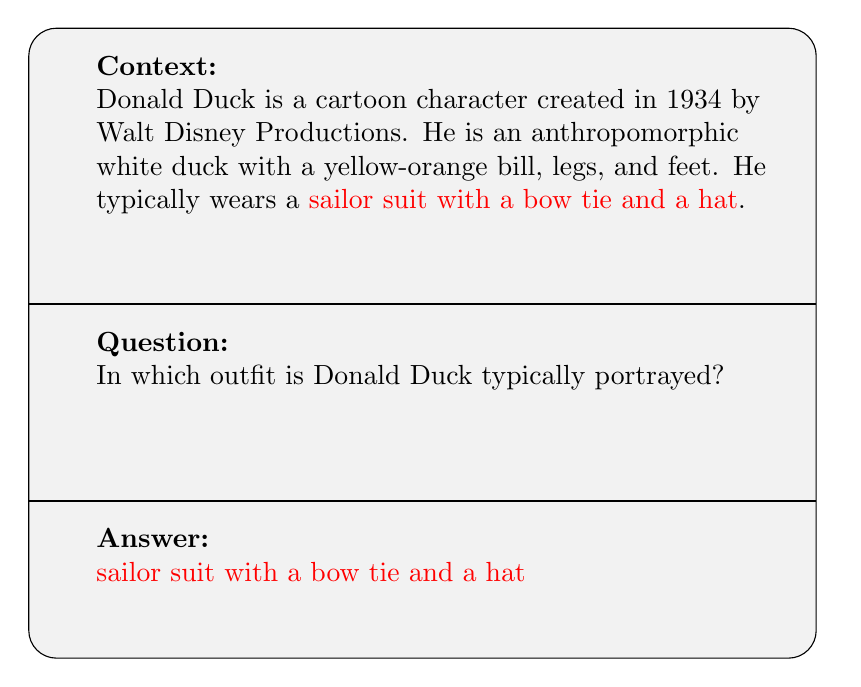
\begin{tikzpicture}
        % Draw paper background
        \draw[fill=gray!10,rounded corners=1em] (0,0) rectangle (10,8);
        % Draw text
        \node[align=left,anchor=north west, text width=9cm,inner sep=1em] at (0.5,8.0) {
            \textbf{Context:}

            Donald Duck is a cartoon character created in 1934 by Walt Disney Productions. He is an anthropomorphic white duck with a yellow-orange bill, legs, and feet. He typically wears a \textcolor{red}{sailor suit with a bow tie and a hat}.
        };
        % Draw a vertical line
        \draw[thick] (0,4.5) -- (10,4.5);
        % Draw question
        \node[align=left,anchor=north west, text width=9cm,inner sep=1em] at (0.5,4.5) {
            \textbf{Question:}

            In which outfit is Donald Duck typically portrayed?
        };
        % Draw a vertical line
        \draw[thick] (0,2.0) -- (10,2.0);
        % Draw question
        \node[align=left,anchor=north west, text width=9cm,inner sep=1em] at (0.5,2.0) {
            \textbf{Answer:}

            \textcolor{red}{sailor suit with a bow tie and a hat}
        };
    \end{tikzpicture}
    \caption{Example of a typical extractive question answering task: The answer span ``sailor suit with a bow tie and a hat'' is highlighted in red in the paragraph.}\label{fig:extractive_qa_example}
\end{figure}
Extractive QA is the task of answering questions given a context containing the answer.
In this context, which can be a short paragraph or an entire Wikipedia article, the correct answer span has to be selected by the model.

One of the most popular datasets for evaluating LLMs in this task is SQuAD~(\cite{rajpurkar:2016:SQuAD}), and its successor SQuAD 2.0~(\cite{rajpurkar:2018:Know}), which includes unanswerable questions in which the correct answer is not present in the context, e.g., ``What are the names of Donald Duck's nephews?'' in the context of the paragraph in Figure~\ref{fig:extractive_qa_example}.
Adding unanswerable questions to the dataset is a way to test the model's ability to detect when a question can not be answered by the given context.
Many other datasets like NarrativeQA~(\cite{kovcisky:2018:The}), QuAC~(\cite{choi:2018:QuAC}) or Natural Questions~(\cite{kwiatkowski:2019:Natural}) are based on the same principle.
They consist of questions written by crowd workers or experts in the field, based on a Wikipedia article snippet or similar text passages.
The exact constraints on the questions and the context vary between the datasets, but the general idea is the same.
Figure~\ref{fig:extractive_qa_example} shows a made-up example of a question and context that could be used in such a dataset.

The evaluation metrics for tasks of this category are based on the overlap between the predicted answer span and the ground truth answer span.
This is called the exact match (EM) score, which measures the percentage of exact matches between the predicted and the ground truth answer span.
Alternatively, the F1 score as the harmonic mean of precision and recall can be used, with precision being defined as
\[ \text{precision} = \frac{\text{number of correct tokens in prediction}}{\text{total number of tokens in the prediction}} \]
and recall as
\[ \text{recall} = \frac{\text{number of correct tokens in prediction}}{\text{total number of tokens in the ground truth}} \]
with a correct token being a predicted token that overlaps with the ground truth answer.
The F1 score is then calculated as
\[ \text{F1} = 2 \times \frac{\text{precision} \times \text{recall}}{\text{precision} + \text{recall}} .\]

Encoder-only LLMs like BERT have to be specifically fine-tuned for the task of extractive QA.
For each token in the provided context, the model assigns a probability of the token being the starting or ending token of the answer span~(\cite{devlin:2018:BERT}).

Decoder-only models like GPT-3 can directly generate the answer from the context and the questions without any fine-tuning, by using the zero-shot, single-shot, or multi-shot capabilities of the model~(\cite{brown:2020:Language}).
In some settings of the datasets, the context can be completely omitted, forcing the model to directly answer the question.
This means that the results of the two approaches are not directly comparable, because even though the models were evaluated on the same dataset, the approaches are fundamentally different.

\subsection{Single and Multiple Choice Question Answering}\label{sec:multiple-choice-qa}
\begin{figure}[tb]
    \centering
    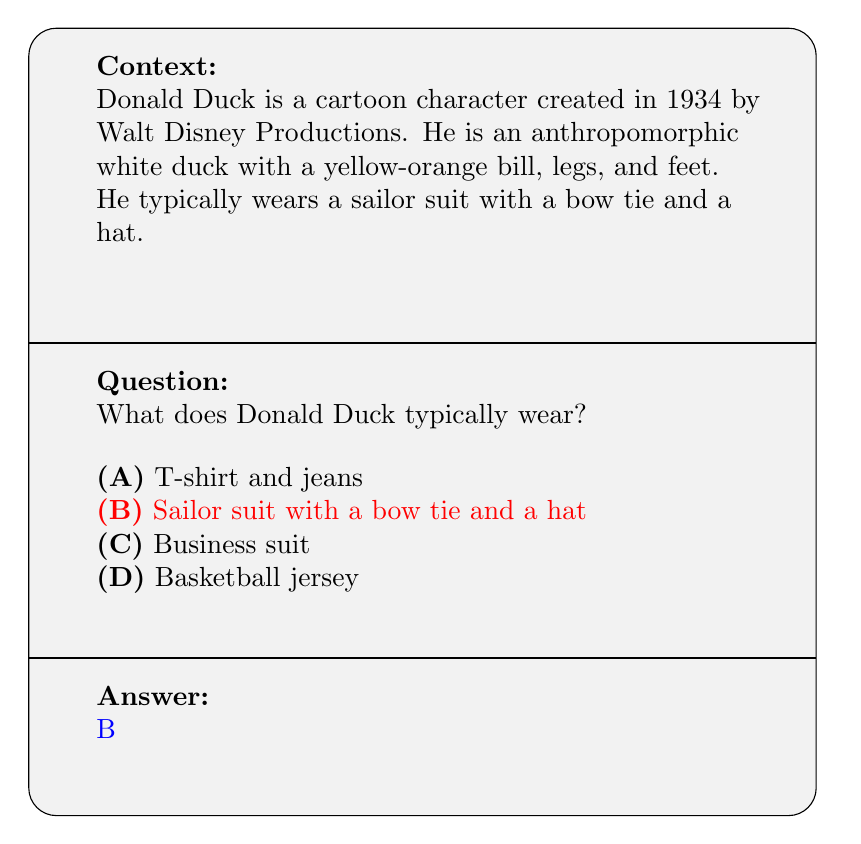
\begin{tikzpicture}
        % Draw paper background
        \draw[fill=gray!10,rounded corners=1em] (0,0) rectangle (10,10);
        % Draw text
        \node[align=left,anchor=north west, text width=8.5cm,inner sep=1em] at (0.5,10.0) {
            \textbf{Context:}

            Donald Duck is a cartoon character created in 1934 by Walt Disney Productions. He is an anthropomorphic white duck with a yellow-orange bill, legs, and feet. He typically wears a sailor suit with a bow tie and a hat.
        };
        % Draw vertical line
        \draw[thick] (0,6) -- (10,6);
        % Draw question
        \node[align=left,anchor=north west, text width=8.5cm,inner sep=1em] at (0.5,6) {
            \textbf{Question:}

            What does Donald Duck typically wear?
        };
        % Draw multiple-choice options
        \node[align=left,anchor=north west, text width=8.5cm,inner sep=1em] at (0.5,4.8) {
            \textbf{(A)} T-shirt and jeans

            \textcolor{red}{\textbf{(B)} Sailor suit with a bow tie and a hat}

            \textbf{(C)} Business suit

            \textbf{(D)} Basketball jersey
        };
        \draw[thick] (0,2) -- (10,2);
        \node[align=left,anchor=north west, text width=9cm,inner sep=1em] at (0.5,2) {
            \textbf{Answer:}

            \textcolor{blue}{B}
        };
    \end{tikzpicture}
    \caption{Example of a single-choice question with context: The correct option is highlighted in red.
    The blue B would be a possible answer generated by the LLM, after being primed with the context and the question.
    }\label{fig:mc_example}
\end{figure}
For single and multiple choice question answering, the model has to select the correct answer from a set of possible answers, which can be done with or without context.
While most datasets are single-choice datasets, some datasets like MultiRC by \cite{khashabi:2018:Looking} are multiple-choice so that the model has to check each answer for correctness, instead of just selecting the best fitting one.
Questions for single and multiple choice QA often stem from official exams, like the MMLU dataset~(\cite{hendrycks:2020:Measuring}), which combines questions from many exams like the United States Medical Licensing Examination or the Examination for Professional Practice in Psychology.
In other datasets, the questions are collected from crowd workers and verified by experts~(\cite{clark:2018:Think},~\cite{mihaylov:2018:Can}).

Figure \ref{fig:mc_example} shows an example of a single-choice question with context.
The LLM is provided with the context, the question and the answer options, and a ``Answer: '' prefix.
Based on this, the model has to select one of the given options.
Evaluation is straightforward in this case, the model's generated answer option is compared to the ground truth answer, and accuracy over all questions is calculated.
For encoder-only models like BERT, this is modeled as a classification task, where the model has to classify the correct answer option from the given options.

\subsection{Long Form Question Answering}\label{sec:long-form-qa}
\begin{figure}[tb]
    \centering
    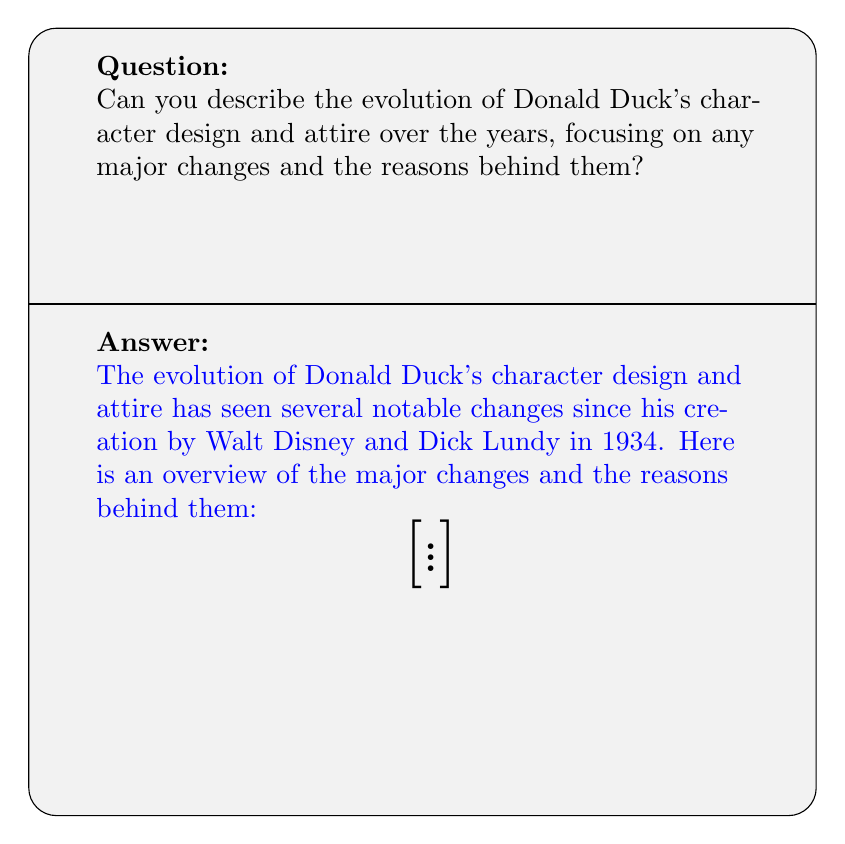
\begin{tikzpicture}
        % Draw paper background for the question
        \draw[fill=gray!10,rounded corners=1em] (0,0) rectangle (10,10);
        % Draw question
        \node[align=left,anchor=north west, text width=8.5cm,inner sep=1em] at (0.5,10) {
            \textbf{Question:}

            Can you describe the evolution of Donald Duck's character design and attire over the years, focusing on any major changes and the reasons behind them?
        };
        % Draw vertical line
        \draw[thick] (0,6.5) -- (10,6.5);
        % Draw sample answer
        \node[align=left,anchor=north west, text width=8.5cm,inner sep=1em] at (0.5,6.5) {
            \textbf{Answer:}

            \textcolor{blue}{The evolution of Donald Duck's character design and attire has seen several notable changes since his creation by Walt Disney and Dick Lundy in 1934. Here is an overview of the major changes and the reasons behind them:}
            

            \centerline{\Huge [\vdots]}
        };
    \end{tikzpicture}
    \caption{Example of LFQA without Context: The question prompts for a detailed answer about Donald Duck's character evolution and attire. The prompt given to the model is written in black, and the sample answer (generated by ChatGPT-3.5) is written in blue. The generated answer continues for multiple paragraphs.}
    \label{fig:long_form_qa_example_with_answer}
\end{figure}
LFQA refers to the task of answering open-ended questions, which can usually not be answered by simply providing one entity or number, but require an in-depth answer.
% Similar tasks exist in the IR community, e.g. generating query-biased summaries as described by \cite{tombros:1998}, in which a retrieval model retrieves and summarizes documents given a user query.
With LLMs being deployed in chatbots and as such expected to deliver answers mostly without context, evaluating the models on LFQA is important.

So far, only a handful of datasets are available for this task, with the first dataset in this category being the ELI5 dataset~(\cite{fan:2019:ELI5}).
It consists of questions and the corresponding highest-voted answer from the ``Explain Like I'm Five'' subreddit, where users ask questions about complex topics, which are then answered by other users.
They are accompanied by support documents, which are retrieved from web sources by querying for the original question.
This dataset was used by~\cite{nakano:2021:Webgpt} to fine-tune GPT-3 for the task of LFQA without using the context documents.
The answers given by the fine-tuned model are evaluated by humans, by comparing them to the highest voted answer from the ELI5 dataset.

\cite{singhal:2023:Towards} use a subset of questions from the multiple-choice dataset MultiMedQA by \cite{singhal:2022:Large} to create a dataset for LFQA.
This dataset consists of about 1200 questions, each of which is accompanied by an answer written by a physician.
To evaluate LLM generated answers on the dataset, the authors let physicians and lay people do pairwise rankings of LLM generated answers versus physician-written answers.
Additionally, the answers were individually rated in multiple rubrics, introduced in a previous work~(\cite{singhal:2022:Large}).

None of the papers for current, main-stream LLMs like GPT-3~(\cite{brown:2020:Language}), GPT-4~(\cite{openai:2023:GPT}) or Llama 2~(\cite{touvron:2023:Llama}) include evaluations on common benchmarks for this category.
This shows that LFQA is still a relatively new task, lacking sufficient academic evaluation measures.

\subsection{Difficulties of Long Form Question Answering}\label{sec:long-form-qa-difficulties}
Recent works by \cite{xu:2023:A} and \cite{krishna:2021:Hurdles} have shown multiple challenges in the task of LFQA, independently of the model architecture used to answer the questions.
Since the answers are free-form text, and not just a multiple choice option, number, or entity, the quality of the model can not be measured using accuracy or similar metrics that require static ground truth information.
Multiple evaluation dimensions are of interest in this thesis:
\begin{itemize}
    \item \textbf{Relevance:} Are the most important aspects of the query answered?
    \item \textbf{Readability:} How easy is the answer to read and understand?
    \item \textbf{Credibility:} Are there any references provided and are they of high quality?
\end{itemize}
This adds additional complexity to the evaluation process, compared to other QA tasks which only measure the correctness of the answer.


\cite{xu:2023:A} survey the evaluation of LFQA, comparing different automatic evaluation methods to human judgment.
They differentiate between general-purpose generation evaluation metrics, which were originally designed for other NLP tasks like summarization or translation, and LFQA-specific metrics.
The following types of metrics are considered general-purpose metrics by \cite{xu:2023:A}:
\begin{itemize}
\item \textbf{Answer-reference metrics:} Include metrics like ROUGE or BERTScore. These metrics compare generated answers to reference answers, focusing on aspects like lexical overlap and semantic similarity.
\item \textbf{Answer-only metrics:} Such as Self-BLEU which measures the fluency and diversity of generated text. These are intrinsic metrics of the generated text and do not need a reference answer for evaluation.
\item \textbf{Question-answer metrics:} Score answers only based on the question without any reference answer. This includes BARTScore by \cite{yuan:2021:bartscore}, which generates a score given the question and the answer.
\item \textbf{Answer-evidence metrics:} Judge the given answer by the evidence from documents used to generate it. This method indirectly assesses the answer's credibility and factual accuracy by comparing the answer to the evidence documents.
\end{itemize}
In addition to these metrics, \cite{xu:2023:A} survey two different versions of LFQA-specific metrics.
The first one is based on Longformer~(\cite{beltagy:2020:Longformer}), in which the model is fine-tuned to produce a score given a question and an answer, optionally combined with evidence documents.
The second model is a fine-tuned version of GPT-3, which is trained to output either \emph{Answer1} or \emph{Answer2} given a question and two answer options.
Both fine-tuned models are trained on the dataset created by \cite{nakano:2021:Webgpt}, which contains human preference labels for different answer pairs.

All automated evaluation methods for LFQA are judged on the task of choosing the preferable answer given two long-form answers to a question.
The results are compared to previous human judgment on the same task.
\cite{xu:2023:A} find that one of their baseline models, choosing always the longest answer, imitates human judgments almost as well as the fine-tuned GPT-3 model, which comes closest to human judgments.
All automated evaluation methods have lower agreement with human judgment than the human annotators have among each other, calculated by pairwise agreement.
This shows that the current automated evaluation methods are not yet able to evaluate LFQA as well as human annotators.

\cite{krishna:2021:Hurdles} investigate the problems of reference-based evaluation metrics like ROUGE-L. 
They highlight that those metrics are unable to capture answer components like examples if those examples are not present in the ground truth answers. 

Furthermore, they note that even human evaluation is limited in judging LFQA over different models.
Some problems include the hiring process of experts, especially when datasets tackle multiple fields of expertise.
Finding experts of similar education and background is challenging when doing evaluations of different models over time, especially for challenging fields like the health domain, as in the dataset used in this thesis.
Additionally, the evaluation process is more mentally demanding for the individual annotator the longer the answers get.
Similar problems have previously been shown by \cite{akoury:2020:Storium} in the context of machine-generated stories.
They find that crowd workers have low Fleiss' kappa agreement for different dimensions like fluency and coherence when evaluating the same stories.
They tackle this problem by using gamification techniques to activate online users of a story-writing platform to evaluate and improve the generated stories, motivating annotators to stay engaged for longer periods of time.
A similar approach is taken by \cite{dugan:2020:RoFT}, who implement a website where users try to differentiate machine-generated text from human-generated text.

We attempt to tackle some issues with evaluating LFQA discussed in this section using the approach presented in this thesis.

\section{Retrieval Models}\label{sec:retrieval-models}
Since we want to use retrieval methods to indirectly evaluate the effectiveness of LLMs in LFQA, we will give some background on the field of information retrieval (IR), and how it relates to LFQA.
IR is concerned with retrieving relevant information based on an information need, from a collection of documents, usually in the form of whole documents, passages, or single sentences.
A brief overview of a typical retrieval pipeline as outlined by \cite{manning:2009:An} is provided and visualized in Figure \ref{fig:reranking_pipeline}.
Given a query, an IR system returns a ranked list of documents that are most relevant to the query.
To achieve this, IR systems estimate a relevance score for each document in the collection with respect to the query.
The documents are then ranked according to their relevance scores, with the most relevant documents appearing at the top of the list.
Some pipelines include a re-ranking step, in which the top-ranked documents are re-ranked after the first retrieval using a more expensive (and ideally more effective) retrieval model.
\begin{figure}[tb]
\centering
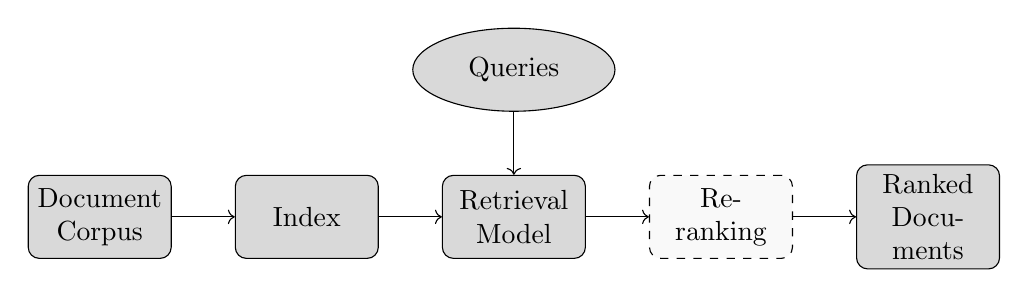
\begin{tikzpicture}[node distance=0.8cm, auto]

% Styles for boxes
\tikzstyle{box} = [rectangle, draw, fill=gray!30, text width=4.5em, text centered, rounded corners, minimum height=3em]
\tikzstyle{user} = [ellipse, draw, fill=gray!30, text width=4.5em, text centered, rounded corners, minimum height=3em]

% Nodes
\node [box, ] (corpus) {Document Corpus};
\node [box,  right=of corpus] (index) {Index};
\node [box,  right=of index] (model) {Retrieval Model};
\node [user, above=of model] (query) {Queries};
\node [box, dashed, fill=gray!5, right=of model] (rerank) {Re-ranking};
\node [box,  right=of rerank] (output) {Ranked Documents};

% Edges
\draw[->] (corpus) -- (index);
\draw[->] (query) -- (model);
\draw[->] (index) -- (model);
\draw[->] (model) -- (rerank);
\draw[->] (rerank) -- (output);

\end{tikzpicture}
\caption{Depiction of a basic retrieval pipeline, with optional re-ranking step. The process begins with a document corpus, which is indexed to facilitate efficient retrieval. Given the information needed by a user in the form of a query, the retrieval model returns the most relevant documents. Optionally, the top-k documents can be re-ranked using a re-ranking model which is usually more resource-intensive.}
\label{fig:reranking_pipeline}
\end{figure}

\subsection{Baseline Retrieval Models}\label{sec:baseline-retrieval-models}
First, we examine the basic retrieval models, which are used as baselines in this thesis.
They have been chosen because they were previously shown to be effective on the dataset used in this thesis~(\cite{goeuriot:2021:Consumer}).
Both models use the implementation in the Terrier IR platform~(\cite{ounis:2005:Terrier}).

\subsubsection{TF-IDF}\label{sec:tf-idf}
Term Frequency-Inverse Document Frequency (tf-idf) is one of the most commonly used models in information retrieval.
It measures the importance of a term in a document relative to a collection of documents or corpus.
The central intuition is that terms that appear frequently in a document but not in many other documents in the corpus are important for the distinguishing the content and thus should be given higher weight.

Given a query \( q \) consisting of terms \( t_1,t_2,\cdots,t_n \) and a document corpus \( D \) of size \( N \), we calculate the score of \( q \) given document \( d \) by first calculating the tf-idf of each term  in \( q \) given \( d \) and then summing them up:
\[ \text{tf-idf}(t, d) = \text{tf}(t, d) \times \text{idf}(t) ,\]
where \( \text{tf}(t, d) \) is the frequency of term \( t \) in document \( d \) and 
\[ \text{idf}(t) = \log \left( \frac{N}{1 + \text{df}(t)} \right), \]
where document frequency \( \text{df}(t) \) is the number of documents containing term \( t \).
The final score of the query given the document is then calculated as
\[ \text{score}(q, d) = \sum_{t \in q} \text{tf-idf}(t, d) .\]
For retrieval given a query \( q \) tf-idf scores are calculated for all documents, which are then ranked according to their score.

In the Terrier IR platform, the implementation of tf-idf uses variants of the tf and idf components.
For Term Frequency, Robertson's tf formulation~(\cite{robertson:2004:Understanding}) is used, which incorporates an additional parameter that adds a saturation effect to the term frequency.
For idf, the original formulation by Sparck Jones~(\cite{sparck:1972:A}) is applied.

\subsubsection{DPH}\label{sec:dph}
Divergence from Randomness (DFR) is a framework in IR that assigns term weights based on the divergence of the actual within-document term frequency distribution from a random term frequency distribution~(\cite{amati:2006:Frequentist}).
The divergence from randomness using the hyper-geometric distribution model (DPH) is one of the models derived from the DFR framework.

The principle behind DFR is that terms that are informative in a document will have a distribution that deviates significantly from what would be expected if terms were distributed randomly.
While TF-IDF emphasizes the importance of terms based on their frequency in a document and their inverse frequency in the corpus, DPH focuses on the divergence of a term's distribution from what would be expected under a random distribution.
Specifically, DPH assesses the divergence using the hyper-geometric distribution.
In essence, where TF-IDF weights terms based on their prominence and rarity, DPH weights them based on how much their occurrence pattern deviates from randomness.
The implementation in the Terrier IR platform follows the original formulation by \cite{amati:2006:Frequentist}.


\subsection{Transformer-based Retrieval Models}\label{sec:transformer-retrieval-models}
As mentioned in earlier sections, transformer-based models have been shown to be effective on a variety of tasks, including IR.
There are different approaches to how transformers can be used for retrieval.
A brief overview of methods used in this thesis is given here.
Transformer models can be used for learning-to-rank, where the model is trained on a dataset to predict which documents are relevant to a query.
This differentiates them from our baseline models, which do not require training.

Two of the most common transformer-based architectures are cross-encoder and bi-encoder models.
\begin{figure}[tb]
  \centering
  % Define colors
%   \definecolor{textcolor}{RGB}{255, 230, 204}
%   \definecolor{encodercolor}{RGB}{204, 229, 255}
%   \definecolor{embeddingcolor}{RGB}{217, 234, 211}
%   \definecolor{scorecolor}{RGB}{230, 204, 255} % New color for scores
  \definecolor{textcolor}{gray}{0.9}
  \definecolor{encodercolor}{gray}{0.9}
  \definecolor{embeddingcolor}{gray}{0.9}
  \definecolor{scorecolor}{gray}{0.9}

  % Bi-Encoder
  \begin{minipage}{.48\textwidth}
    \centering
    \begin{tikzpicture}[node distance=0.7cm, auto, every node/.style={scale=0.8}]
      \tikzstyle{text_in} = [rectangle, rounded corners, minimum width=3cm, minimum height=1cm, align=center, draw=black, fill=textcolor]
      \tikzstyle{encoder} = [rectangle, rounded corners, minimum width=3cm, minimum height=1cm, align=center, draw=black, fill=encodercolor]
      \tikzstyle{embedding} = [rectangle, rounded corners, minimum width=3cm, minimum height=1cm, align=center, draw=black, fill=embeddingcolor]
      \tikzstyle{score} = [ellipse, minimum width=2cm, minimum height=1cm, align=center, draw=black, fill=scorecolor]
      \tikzstyle{highlight}= [draw=black, rounded corners, inner sep=1cm, dashed, thick]
      % Nodes
      \node[text_in] (query) {Query};
      \node[encoder, below=of query] (qencoder) {Query Encoder};
      \node[embedding, below=of qencoder] (qembed) {Query Embedding};
      
      \node[text_in, right=of query, xshift=1cm] (doc) {Document};
      \node[encoder, below=of doc] (docencoder) {Doc Encoder};
      \node[embedding, below=of docencoder] (docembed) {Doc Embedding};

      \node[score, below=of qembed.south, xshift=2.5cm] (biScore) {Relevance Score}; % New node for relevance score


        % draw highlight box around document, doc encoder and doc embeddings. Label above the box says "Offline"
        \node[highlight, fit=(doc) (docencoder) (docembed), label={[align=center]above:Offline}] (docbox) {};

      % Arrows
      \draw[-{Latex[length=3mm]}] (query) -- (qencoder);
      \draw[-{Latex[length=3mm]}] (qencoder) -- (qembed);
      \draw[-{Latex[length=3mm]}] (qembed) -- (biScore);
      \draw[-{Latex[length=3mm]}] (doc) -- (docencoder);
      \draw[-{Latex[length=3mm]}] (docencoder) -- (docembed);
      \draw[-{Latex[length=3mm]}] (docembed) -- (biScore);

    \end{tikzpicture}
    \caption{Bi-Encoder Architecture. Query and document are encoded separately, document embeddings can be calculated offline. Then the relevance is calculated as the similarity between the embeddings.}
    \label{fig:bi-encoder}
  \end{minipage}
  \hfill
  % Cross-Encoder
  \begin{minipage}{.48\textwidth}
    \centering
    \begin{tikzpicture}[node distance=0.7cm, auto, every node/.style={scale=0.8}]
      \tikzstyle{text_in} = [rectangle, rounded corners, minimum width=3cm, minimum height=1cm, align=center, draw=black, fill=textcolor]
      \tikzstyle{encoder} = [rectangle, rounded corners, minimum width=3cm, minimum height=1cm, align=center, draw=black, fill=encodercolor]
      \tikzstyle{embedding} = [rectangle, rounded corners, minimum width=3cm, minimum height=1cm, align=center, draw=black, fill=embeddingcolor]
      \tikzstyle{score} = [ellipse, minimum width=2cm, minimum height=1cm, align=center, draw=black, fill=scorecolor]

      % Nodes
      \node[text_in, right=] (query) {Query};

      \node[text_in, right=of query, xshift=1cm] (doc) {Document};

      \node[text_in, below=of query.south, xshift=2.5cm] (qdoc) {Query $+$ Document};

      \node[encoder, below=of qdoc] (qencoder) {Cross-Encoder};

      \node[score, below=of qencoder] (biScore) {Relevance Score};
      % Arrows
      \draw[-{Latex[length=3mm]}] (query) -- (qdoc);
      \draw[-{Latex[length=3mm]}]  (doc) -- (qdoc);
      \draw[-{Latex[length=3mm]}] (qdoc) -- (qencoder);
      \draw[-{Latex[length=3mm]}] (qencoder) -- (biScore);

    \end{tikzpicture}
    \caption{Cross-Encoder Architecture. Query and document are first concatenated and then fed to a single encoder model, the relevance is calculated by a linear layer on top of the encoder.}
    \label{fig:cross-encoder}
  \end{minipage}
\end{figure}
Bi-encoders independently embed queries and documents using transformer models like BERT~(\cite{devlin:2018:BERT}).
For the document collection, this can be done offline since the embeddings are independent of the query.
This separation allows them to efficiently process large datasets as the embeddings for the documents can be pre-computed and stored.
It also enables efficient retrieval, since at inference time only the embedding for the current query has to be calculated and compared to the pre-computed document embeddings.
The documents are then ranked according to their embedding similarity to the query.

Cross-encoders, on the other hand, take a concatenated input sequence of both query and document and produce a scalar relevance score.
This joint modeling enables them to better capture the interaction between a query and a document by leveraging the transformer's attention mechanism.
Due to their fine-grained interaction modeling, cross-encoders are more effective than bi-encoders in terms of precision in retrieving relevant documents as shown by \cite{thakur:2020:Augmented} and \cite{rosa:2022:In}.
However, the need to process each query-document pair individually makes them computationally demanding, especially for large datasets.
As a result, they are typically only used in second-stage retrieval, where the objective is to re-rank the top results obtained from an initial retrieval method.

The following sections describe the different transformer-based retrieval models used in this thesis.
\subsubsection{monoT5 + duoT5}\label{sec:monoT5-duoT5}
\cite{roberts:2019:Exploring} introduce monoT5 and duoT5, which are based on previous work by \cite{nogueira:2019:Multi}, who introduced monoBERT and duoBERT, first applying transformer architecture to the task of document ranking.
The general idea is to first use a baseline retrieval model like BM25 to retrieve an initial set of relevant documents.
Then, pairs of the query and each document in the initial set are concatenated and fed into the mono version of the transformer model, which produces a scalar score for each query-document pair.
The documents with the highest scores are then fed into the duo model, which takes the query and each possible pair of documents as input, outputting a probability of one document being more relevant than the other.
Given those scores, the documents are re-ranked another time, serving as the final output of the retrieval pipeline.
The main difference between the BERT and T5 versions is that for BERT the [CLS] token can be used as input to a single-layer neural network to output a probability of the document being relevant.
Since there is no [CLS] token for models in the T5 family, as they are sequence-to-sequence models, this part is done using an input template:
\begin{equation}
    \text{Query: \emph{q} Document: \emph{d} Relevant:}
\end{equation} 
where the model is fine-tuned to produce the token \emph{true} or \emph{false} given query \emph{q} and document \emph{d}.

At inference, softmax is applied to the \emph{true} and \emph{false} tokens only, the scores are then calculated using the probability of the \emph{true} token.
This works analogously for the Duo version of both models, by just adding the second document.
Both monoT5 and duoT5  belong to the family of cross-encoder models, sharing the general characteristics of those models.

This model architecture allows for precisely tuning retrieval efficiency vs. effectiveness, by parameterizing how many documents are filtered in each step, making the model suitable for different use cases.


\subsubsection{ColBERT}\label{sec:colbert}
\begin{figure}[tb]
\centering
% Define colors
% \definecolor{textcolor}{RGB}{255, 230, 204}
% \definecolor{encodercolor}{RGB}{204, 229, 255}
% \definecolor{embeddingcolor}{RGB}{217, 234, 211}
% \definecolor{similaritycolor}{RGB}{255, 204, 204} % New color for similarity scores
% \definecolor{scorecolor}{RGB}{230, 204, 255} % New color for scores

\definecolor{textcolor}{gray}{0.9}
\definecolor{encodercolor}{gray}{0.9}
\definecolor{embeddingcolor}{gray}{0.9}
\definecolor{scorecolor}{gray}{0.9}
\definecolor{similaritycolor}{gray}{0.9}
% ColBERT Retrieval Model
\begin{tikzpicture}[node distance=0.7cm, auto, every node/.style={scale=0.8}]
\tikzstyle{text_in} = [rectangle, rounded corners, minimum width=3cm, minimum height=1cm, align=center, draw=black, fill=textcolor]
\tikzstyle{token} = [rectangle, rounded corners, minimum width=0.5cm, minimum height=1cm, align=center, draw=black, fill=textcolor]
\tikzstyle{encoder} = [rectangle, rounded corners, minimum width=3cm, minimum height=1cm, align=center, draw=black, fill=encodercolor]
\tikzstyle{embedding} = [rectangle, rounded corners, minimum width=0.5cm, minimum height=1cm, align=center, draw=black, fill=embeddingcolor]
\tikzstyle{similarity} = [ellipse, minimum width=1cm, minimum height=1cm, align=center, draw=black, fill=similaritycolor]
\tikzstyle{score} = [ellipse, minimum width=2cm, minimum height=1cm, align=center, draw=black, fill=scorecolor]
% black thick dotted border around document, doc encoder and doc embeddings
\tikzstyle{highlight}= [draw=black, rounded corners, inner sep=1cm, dashed, thick]

\node[text_in] (query) {Query};
\node[token, below=of query, xshift=-1cm] (q1) {};
\node[token, below=of query] (q2) {};
\node[token, below=of query, xshift=1cm] (q3) {};
\node[encoder, below=of q2] (qencoder) {Query Encoder};
\node[embedding, below=of qencoder, xshift=-1cm] (qe1) {};
\node[embedding, below=of qencoder] (qe2) {};
\node[embedding, below=of qencoder, xshift=1cm] (qe3) {};

\node[text_in, right=of query, xshift=3cm] (doc) {Document};
\node[token, below=of doc, xshift=-1cm] (d1) {};
\node[token, below=of doc] (d2) {};
\node[token, below=of doc, xshift=1cm] (d3) {};
\node[encoder, below=of d2] (docencoder) {Doc Encoder};
\node[embedding, below=of docencoder, xshift=-1cm] (de1) {};
\node[embedding, below=of docencoder] (de2) {};
\node[embedding, below=of docencoder, xshift=1cm] (de3) {};

\node[similarity, below=of qe2.south] (maxSim1) {MaxSim};
\node[similarity, below=of qe2.south, xshift=3.5cm] (maxSim2) {MaxSim};
\node[similarity, below=of de2.south] (maxSim3) {MaxSim};

\node[score, below=of maxSim2] (score1) {Sum};

% draw highlight box around document, doc encoder and doc embeddings. Label above the box says "Offline"
\node[highlight, fit=(doc) (docencoder) (de1) (de2) (de3), label={[align=center]above:Offline}] (docbox) {};

% Arrows
\draw[-{Latex[length=3mm]}] ([xshift=-0.8cm]query.south) -- (q1.north);
\draw[-{Latex[length=3mm]}] (query.south) -- (q2.north);
\draw[-{Latex[length=3mm]}] ([xshift=0.8cm]query.south) -- (q3.north);
\draw[-{Latex[length=3mm]}] (q1.south) -- ([xshift=-0.8cm]qencoder.north);
\draw[-{Latex[length=3mm]}] (q2.south) -- (qencoder.north);
\draw[-{Latex[length=3mm]}] (q3.south) -- ([xshift=0.8cm]qencoder.north);
\draw[-{Latex[length=3mm]}] ([xshift=-0.8cm]qencoder.south) -- (qe1.north);
\draw[-{Latex[length=3mm]}] (qencoder.south) -- (qe2.north);
\draw[-{Latex[length=3mm]}] ([xshift=0.8cm]qencoder.south) -- (qe3.north);
\draw[-{Latex[length=3mm]}] ([xshift=-0.8cm]doc.south) -- (d1.north);
\draw[-{Latex[length=3mm]}] (doc.south) -- (d2.north);
\draw[-{Latex[length=3mm]}] ([xshift=0.8cm]doc.south) -- (d3.north);
\draw[-{Latex[length=3mm]}] (d1.south) -- ([xshift=-0.8cm]docencoder.north);
\draw[-{Latex[length=3mm]}] (d2.south) -- (docencoder.north);
\draw[-{Latex[length=3mm]}] (d3.south) -- ([xshift=0.8cm]docencoder.north);
\draw[-{Latex[length=3mm]}] ([xshift=-0.8cm]docencoder.south) -- (de1.north);
\draw[-{Latex[length=3mm]}] (docencoder.south) -- (de2.north);
\draw[-{Latex[length=3mm]}] ([xshift=0.8cm]docencoder.south) -- (de3.north);
% draw dotted arrows from query and document to maxSim1, maxSim2 and maxSim3
\draw[-{Latex[length=3mm]}] (qe1.south) -- (maxSim1);
\draw[-{Latex[length=3mm]}] (qe2.south) -- (maxSim2);
\draw[-{Latex[length=3mm]}] (qe3.south) -- (maxSim3);
\draw[-{Latex[length=3mm]}, dashed] (de1.south) -- (maxSim1);
\draw[-{Latex[length=3mm]}, dashed] (de1.south) -- (maxSim2);
\draw[-{Latex[length=3mm]}, dashed] (de1.south) -- (maxSim3);
\draw[-{Latex[length=3mm]}, dashed] (de2.south) -- (maxSim1);
\draw[-{Latex[length=3mm]}, dashed] (de2.south) -- (maxSim2);
\draw[-{Latex[length=3mm]}, dashed] (de2.south) -- (maxSim3);
\draw[-{Latex[length=3mm]}, dashed] (de3.south) -- (maxSim1);
\draw[-{Latex[length=3mm]}, dashed] (de3.south) -- (maxSim2);
\draw[-{Latex[length=3mm]}, dashed] (de3.south) -- (maxSim3);
\draw[-{Latex[length=3mm]}] (maxSim1.south) -- (score1);
\draw[-{Latex[length=3mm]}] (maxSim2.south) -- (score1);
\draw[-{Latex[length=3mm]}] (maxSim3.south) -- (score1);
\end{tikzpicture}
\caption{ColBERT Retrieval Model. The query and document are processed separately to generate token embeddings. The maximum cosine similarity between all token embeddings of the query and document is calculated and summed over all query tokens, which is the relevance score of the document given the query.}
\label{fig:colbert}
\end{figure}
ColBERT~(\cite{khattab:2020:Colbert}) is another BERT-based model for document ranking.
It shares similarities with the general bi-encoder architecture but introduces some modifications to improve effectiveness.
Instead of representing each document and query as a single vector (e.g. the [CLS] token), ColBERT uses the contextualized embeddings for each token in the document or query.
For the documents, embedding can again be done offline, so that at the retrieval stage, only the embeddings for the query have to be generated and compared to the documents.
The relevance score for document $d$ given query $q$ is estimated using their late interaction model, in which maximum cosine similarity between all query term embeddings and document term embeddings is calculated, and then summed over for all query terms.
This architecture combines the advantages of bi-encoders and cross-encoders, as it is computationally efficient using the offline embeddings for the documents, while also capturing the interaction between query and document using the contextualized embeddings similar to cross-encoders.

The ColBERT architecture can be used for re-ranking or end-to-end retrieval.
In the second case, an additional step is added in which the complete collection is filtered for relevant documents using similarity search to find documents that contain similar terms as the query.
In the second step, the remaining documents are re-ranked using the maximum similarity metrics.

\subsubsection{ColBERTv2}\label{sec:colbertv2}
ColBERTv2~\citep{santhanam:2021:Colbertv2} is directly based on the late-interaction architecture of ColBERT but adds improvements to the architecture and the training process.

To improve the training process, a new process of generating hard negatives is applied, in which a cross-encoder model is used to first rank passages given a query.
From the ranked passages a highly ranked one is selected as the positive passage and a low ranked one as the negative passage.

Improvements to the architecture are made by incorporating a residual compression technique.
While for ColBERTv1 each token embedding is saved separately in its original state, ColBERTv2 represents each token embedding as its nearest neighboring centroid embedding and a residual.
The centroids are calculated using k-means clustering on the token embeddings of a sample of all passages at indexing time. 
This allows for a more compact representation of the token embeddings since only the centroid embedding has to be stored.

As shown by the authors, ColBERTv2 is more effective than ColBERTv1 on all evaluated datasets, while also being more efficient

\subsection{Evaluation of Retrieval Models}\label{sec:evaluation-of-retrieval-models}
Evaluation metrics are important for the automatic evaluation of retrieval model effectiveness.
They provide a quantitative measure of how well a system retrieves relevant documents in response to a user's query.
To be able to evaluate different retrieval methods, relevance assessments for document-query pairs have to be defined by human assessors.

There are multiple metrics which can be used in information retrieval tasks:
\begin{itemize}
    \item \textbf{Precision}: Captures the fraction of retrieved documents that are relevant.
    \item \textbf{Recall}: Captures the fraction of relevant documents that are retrieved.
    \item \textbf{F1 Score}: The harmonic mean of precision and recall.
    \item \textbf{Mean Average Precision (MAP)}: The arithmetic mean of each query's average precision at each document position in a ranking.
    \item \textbf{Normalized Discounted Cumulative Gain (nDCG)}: Considers both the ranking and the relevance grade of retrieved documents, weighing highly relevant documents higher than less relevant ones, assigning a higher information gain for documents that are ranked higher.
\end{itemize}
Given the context of the dataset used in this thesis, which contains multiple queries with documents assessed for relevance between 0 and 3, the nDCG metric is the most suitable one.

The formula for nDCG@k is as follows is based on the concept of cumulative gain (CG), which is the sum of the relevance ratings of all documents up until position k:
\[ \text{CG@k} = \sum_{i=1}^{k} r(d_i,q) ,\]
where $r(d_i,q)$ is the relevance rating of document $d_i$ for query $q$.
Based on that, the discounted cumulative gain (DCG) is defined as
\[ \text{DCG@k} = \sum_{i=1}^{k} \frac{r(d_i,q)}{\log_2(i+1)} ,\]
where the relevance ratings are discounted by the logarithm of the rank of the document, to weight higher-ranked documents more than lower-ranked ones.
The ideal DCG (IDCG) is the DCG of the ideal ranking, which is the ranking of documents sorted descending by their relevance rating.
This produces the highest possible DCG for a set of retrieved documents.
Finally, the normalized DCG is calculated as
\[ \text{nDCG@k} = \frac{\text{DCG@k}}{\text{IDCG@k}} \]
which normalizes the DCG by the IDCG, producing a score between 0 and 1.
The cutoff value of $k$ is set depending on how many of the ranked documents should be considered for each query.

\subsection{Using Retrieval Models for Evaluating NLP tasks}\label{sec:eval-mts-ir}
When evaluating Natural Language Processing (NLP) tasks, IR techniques have been mainly used to evaluate machine translation systems.
Since both question answering and machine translation are sequence-to-sequence tasks with multiple possible correct answers, there are similarities in the evaluation setup.

For machine translation, a model is given a source sentence and has to produce a target sentence in another language.
Those systems are usually evaluated given a ground truth reference sentence, which is compared to the predicted sentence.
Traditionally, methods like BLEU~(\cite{papineni:2002:Bleu}), ROUGE~(\cite{lin:2004:Rouge}), or METEOR~(\cite{banerjee:2005:METEOR}) are used to compare the predicted sentence to one or multiple reference sentences.
There are multiple versions of those metrics with slightly different parameters, which mostly differ in what sequences of tokens are compared (1-gram, 2-gram, 3-gram, 4-gram, longest common sub-sequence), how precision and recall are weighted, and how the results are smoothed.
In the end, all of those metrics produce a similarity score between the predicted and the reference sentence, which can be used to compare different models.

Alternative approaches incorporating ranking methods have been proposed as well.
\cite{duh:2008:Ranking} argues that, considering the final goal is to compare different translation systems, a direct comparison between the systems is preferable to evaluating their quality individually.
He shows that ranking methods like RankSVM~(\cite{joachims:2002:Optimizing}) and RankBoost~(\cite{freund:2003:An}) can be applied to rank different candidate translations against the reference, producing similar scores to the BLEU baseline on the same feature set.
When incorporating intra-set features like the binary ``highest BLEU score in set'', which can not easily be incorporated into BLEU-like scores, the ranking methods achieve higher similarities to human rankings compared to BLEU and smoothed BLEU.

Another approach based on learning-to-rank methods is proposed by \cite{li:2013:Listwise}.
Again, they compare multiple translation candidates to a reference sentence, but here they use listwise learning-to-rank methods to generate a ranking of the candidates.
The objective of listwise ranking is to train a ranking function that minimizes the loss between the predicted ranking and the ground truth human-generated ranking on a training set.
Similar to \cite{duh:2008:Ranking}, they show that the ranking-based methods correlate stronger with human judgment, compared to BLEU-like metrics which show lower correlation.

\cite{guzman:2019:Pairwise} use neural methods to incorporate syntactic and semantic information into the evaluation process.
They train a pairwise ranking model, which compares two candidate sentences given the reference and returns which one is the better translation.
Even though they are not more effective than other state-of-the-art methods in terms of agreeing with human judgments, they deliver competitive results while staying closer to the human evaluation framework.


This overview shows that information retrieval methods have successfully been applied to the task of evaluating machine translation systems.
However, those approaches are hard to transfer to the task of evaluating from question-answering systems, since the evaluation metrics are not directly applicable.
All ranking-based machine translation evaluation methods mentioned here compare the set of candidate translations to a single reference translation, trying to rank the candidate translations among each other.
Since the space of correct answers given a long-form question is generally much higher in comparison to translating a sentence, this evaluation setup can not be directly applied here.
So, even though information retrieval methods are applied here as well, the evaluation approach is formulated differently.

\section{Summary}
In this chapter, we presented an overview of the current state of research for evaluating LLMs for question answering.
We highlighted that the evaluation of LFQA is challenging since the answers are free-form text and not just a single entity, number, or multiple choice option.
Additionally, we show that evaluating long-form answers in one single dimension of correctness is not sufficient, as other aspects like readability and credibility are important as well.
In this thesis, we tackle both of the mentioned challenges.

Based on the assumption that if we develop a ranking model that can effectively rank human-generated documents in the dimensions of relevance, readability, and credibility in a way that is similar to human judgment, we can use the ranking model to evaluate LFQA systems.
The evaluation of text generated by LLMs can be done by ranking the LLM output with the previously validated retrieval model and using the rank of the generated output alongside human-written texts as a proxy for the effectiveness of the generated answer.
We formalize this approach as follows:
\begin{enumerate}
    \item \textbf{Dataset acquisition:} Collect a dataset of queries \( q_1, q_2, \ldots, q_n \) with associated human-generated documents for each query \( d_{i,1}, d_{i,2}, \ldots d_{i,j} \forall i \in \{1, \ldots, n\} \). Each document has a relevance rating \( r_{rel}(d_{i,j}, q_i) \), a readability rating \( r_{read}(d_{i,j}, q_i) \) and a credibility rating \( r_{cred}(d_{i,j}, q_i) \) for the query.
    \item \textbf{Retrieval Model Evaluation:} Evaluate a set of retrieval models \( \mathcal{M}\) on the dataset, using the nDCG metric for relevance, readability and credibility.
    \item \textbf{Generate LLM Answers:} Use a set of LLMs \( \mathcal{L} \) to generate answers \( a_{l,i} \) for all queries \( q_i \).
    \item \textbf{Rank Answers:} Add the generated answers \( a_{l,i} \) to the documents \(d_{1,i}, d_{2,i}, \cdots, d_{n,i} \) for each query \( q_i \) and rank them using the best of the previously evaluated retrieval model from set \( \mathcal{M} \).
\end{enumerate}
This approach allows us to evaluate the capabilities of multiple LLMs in LFQA, by comparing the ranks of the generated answers as a proxy for their quality.
By evaluating the retrieval models on multiple evaluation criteria, we tackle the problem of evaluating the answers in multiple dimensions.
% \chapter{Experimental Setup}
This chapter describes the experimental setup of this thesis, including the data collection and preparation, the retrieval pipeline development and the generation of LLM responses.

\section{Overview}\label{sec:overview}
The final goal of this project is to have a pipeline with which the answers of different LLMs can be ranked, in comparison to human answers.
This means, we first need a dataset, consisting of questions as well as human answers to these questions.
Those human generated answers need to be ranked according to how well they answer the given question.
Then, we need to develop a retrieval pipeline, which is able to retrieve the best answer to a given question in accordance to the ranking of the human answers.
Finally, the answers generated by different LLMs can be ranked using the developed retrieval pipeline.
\\\\
This allows us to compare long form question answering capabilities between different LLMs or between different prompting strategies for the same LLM.
Additionally, an expected range of performance for a given LLM can be established, given that the answer of a LLM differs every time it is prompted with the same question.
\\\\
To be able to do this, we first need to collect a suitable dataset, since a benchmark like this has not been formulated before.
Then, different retrieval methods have to be compared on the dataset, to find the best performing one.
Finally, the LLMs have to be selected, and the answers generated by them have to be ranked using the best retrieval method.
\\
This process is described in detail in the following sections.

\section{Data Collection and Preparation}\label{sec:dataset}
The used dataset is based on the test set of the CLEF eHealth 2021 dataset \cite{goeuriot:2021}.
It was originally intended to evaluate the ability of retrieval systems to provide credible, readable and relevant answers to laypersons' health questions.

\subsection{CLEF eHealth 2021 Dataset}
The test set consists of 55 health related queries, which either stem from Reddit or Google search trends.
While the Reddit-sourced queries are well-formulated questions about specific health topics, the queries from Google search trends are not necessarily phrased as questions but rather as classical search queries.
\\
In addition to the queries, the dataset includes a collection of web documents and social media content.
The web documents were mainly obtained from the CommonCrawl archive, encompassing a diverse range of 600 domains.
This list of domains was created by executing medical queries via Microsoft Bing API and was augmented by adding known reliable and unreliable health-related websites.
The dataset was expanded by incorporating social media comments and posts from Reddit and Twitter.
These were collected by manually generating search queries based on 150 pre-selected health topics and retrieving relevant posts and comments from these platforms.
\\
To get evaluations in each of the three categories (credible, readable and relevant), each query was assigned 250 documents based on rank-biased precision (RBP)-based Method A~(\cite{moffat:2008}).
RBPA is a method for choosing which documents from a pool of documents to select for evaluation by human annotators.
The pool of documents in this case is the collection of web documents and social media content returned by the participating teams of the shared task, as well as the organizer's baseline systems.
From this, documents are evaluated based on their rank in different runs, and then scored according to different metrics.
A more detailed description of the pooling method can be found in \cite{lipani:2017}.
\\
After the 250 documents per query are selected, the documents are evaluated by humans for credibility, readability and relevance.
In total, there are 26 annotators, each annotating documents for between 1 and 4 queries completely.
The annotators were not medical experts, but received written training material.
In the end, annotations were made for  a total of $11 357$ unique documents.
This differs from the total amount of annotations which is $12 500$, since some documents were annotated multiple times but for different queries.
\\
The annotations for relevance and readability are in the categories 0 (not relevant/readable), 1 (somewhat relevant/readable) and 2 (highly relevant/credible).
For scoring credibility, a category 3 exists, which is also interpreted as highly credible.
A reasoning for this is not given in the original paper.
\\\\
How the adapted dataset is created from the original dataset is described in the following section.
\subsection{Dataset Collection}
There are two ways of accessing the CLEF eHealth 2021 dataset.
\\
Option one is to download the indexed collection directly.
This index does not contain the full text of the documents, so it can't be used to compare the original documents against newly generated answers.
\\
The second option is to access all documents individually, given their IDs.
This is in easily done in theory, by using the provided scripts in the organizer's GitHub repository\footnote{\url{https://github.com/CLEFeHealth/CHS-2021}}.
Scripts are provided to download the documents from the CommonCrawl archive, as well as the social media content directly over the respective APIs.
\\
Unfortunately, with Twitter shutting down their free tier of the API, in the beginning of April 2023, this is now only possible with a prohibitively expensive paid tier.
\\
For Reddit, those API changes followed just a few months later, making it impossible to download the social media content from Reddit as well.
Even tough we started downloading some Reddit content before those changes, the already slow access to the Reddit data did not allow for downloading all content in time.
\\
This was unfortunate timing, but since the organizers of the CLEF eHealth task reported in their paper that the human credibility assessments of social media documents were significantly lower than those of web documents, we decided to only use the web documents for our dataset.
The web documents are easily accessible via the CommonCrawl archive.
\\
\\
Before accessing all relevant documents from the CommonCrawl archives, the list of documents was filtered to only include documents which were annotated for at least one query.
Discarding all documents from Reddit and Twitter, as well as web documents which were not assessed for any query, resulted in a total of $6692$ documents downloaded from the CommonCrawl archive using a slightly modified version of the provided script.
This provides us with WARC files for the relevant documents.
\\
Since all social media content was discarded, the number of queries for which documents are available is reduced to 50, since of the total 55 queries, 5 queries only have social media content associated with them.

\subsection{Preprocessing}
The files in the WARC format contain the full HTML of the web documents.
Before being able to compare the content to the generated answers, the HTML is extracted from the documents.
HTML elements containing fewer than 50 characters in the elements body are discarded, assuming they are not relevant for the content of the document (e.g. fields of navigation bars).
Then, the plain text is extracted using the ChatNoir Resiliparse Library\footnote{\url{https://resiliparse.chatnoir.eu/en/stable/}}.
\\
The final dataset now consists of 50 queries, each of which has between 39 and 249 documents associated with it that are evaluated for relevance, readability and credibility.


\section{Retrieval Pipeline Development}
In this section, the implementation of the different retrieval pipelines is discussed.
The baseline models (DPH and TF-IDF), as well as the ColBERT version 1 and the monoT5/duoT5 based pipelines are implemented in the PyTerrier framework by \cite{pyterrier:2020}, which is a Python API for the Terrier IR Platform~(\cite{macdonald:2012}).
The ColBERT version 2 pipeline is based on the original implementation provided by the authors\footnote{\url{https://github.com/stanford-futuredata/ColBERT}}.
\\
Those pipelines are all designed to retrieve the most relevant documents for a given query.
Since our dataset also contains annotations for readability and credibility, we also want to be able to retrieve documents based on those criteria.
To extend the retrieval pipelines for those metrics, we experiment with adding external scores to the retrieval process.
This is described in section \ref{sec:external-scores}.
\\

\subsection{Retrieval Setup}
The retrieval setup in this work differs from the usual retrieval setup, in which a large document collection is indexed, and then multiple queries are run against the index using different retrieval models.
In our case, we build separate indices for each query, containing only the documents that are evaluated for that query.
This ensures that each document that is retrieved for a query is also evaluated for that query.

\subsection{Baseline Models}
\begin{figure}
    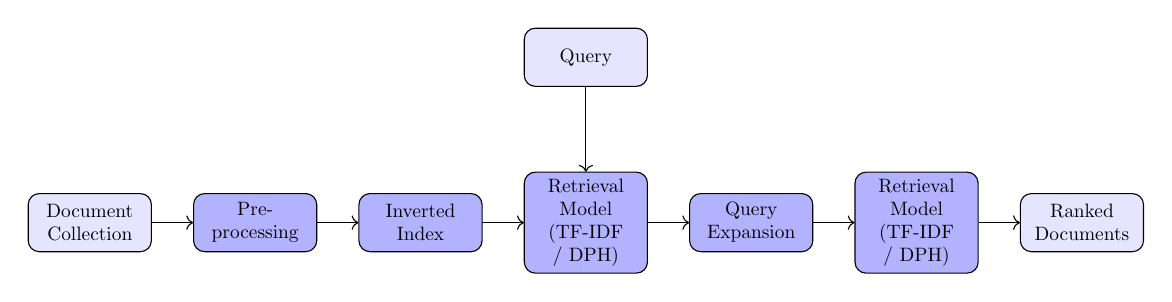
\begin{tikzpicture}[node distance=3cm, every node/.style={scale=0.7}]
    \tikzstyle{box} = [rectangle, draw, fill=blue!10,  text width=2cm, text centered, rounded corners, minimum height=3em]
    \tikzstyle{process} = [rectangle, draw, fill=blue!30,  text width=2cm, text centered, rounded corners, minimum height=3em]
    \node (docCol) [box] {Document Collection};
    \node (preprocess) [process, right of=docCol] {Pre-\\processing};
    \node (invertedindex) [process, right of=preprocess] {Inverted Index};
    \node (retrieval) [process, right of=invertedindex] {Retrieval Model (TF-IDF / DPH)};
    \node (qe) [process, right of=retrieval] {Query Expansion};
    \node (reranking) [process, right of=qe] {Retrieval Model (TF-IDF / DPH)};
    \node (ranked) [box, right of=reranking] {Ranked Documents};
    \node (query) [box, above of=retrieval] {Query};

    \draw [->] (docCol) -- (preprocess);
    \draw [->] (preprocess) -- (invertedindex);
    \draw [->] (invertedindex) -- (retrieval);
    \draw [->] (retrieval) -- (qe);
    \draw [->] (qe) -- (reranking);
    \draw [->] (reranking) -- (ranked);
    \draw [->] (query) -- (retrieval);

    \end{tikzpicture}
\caption{Baseline retrieval pipeline, using either TF-IDF or DPH as retrieval model as well as query expansion.}
\label{fig:baseline-pipeline}
\end{figure}


This section describes the implementation of the baseline models, namely DPH and TF-IDF.
For both models, the basic indexing function of PyTerrier is used, which indexes and preprocesses the documents.
Preprocessing is done with the default values, which includes the following operations:
\begin{itemize}
    \item{\textbf{Tokenization}, using the default PyTerrier tokenizer, which splits on non-alphanumeric characters. Additional rules to discard tokens which are longer than 20 characters, contain more than 4 digits, or contain the same character more than 3 times in a row are applied. All tokens are also converted to lowercase.}
    \item \textbf{Stopword removal}, using the default PyTerrier stopword list.
    \item \textbf{Stemming}, using the Porter stemmer, a rule-based stemmer.
\end{itemize}
The resulting inverted index contains all remaining tokens, and a mapping from each token to the documents in which it occurs.
\\
The two retrieval models TF-IDF and DPH are then applied using the default parameters.
More details about the models can be found in section \ref{sec:baseline-retrieval-models}.
\\
\\
Both models are tested with and without query expansion.
We use BO1 query expansion, which is a query expansion method that uses the documents retrieved by the original query to expand the query.
It adds terms from the retrieved documents to the original query based on informativeness, which is a measure of how frequently the term occurs in the documents compared to how frequently it occurs in the whole collection.
Terms that occur more frequently in the retrieved documents than in the collection are added to the query.
Afterwards, the expanded query is run against the index again, and the documents are ranked according to the new query.
\\
\\
The resulting pipeline is shown in figure \ref{fig:baseline-pipeline}.
This produces a ranked list of documents for each query, which can then be compared to the order of documents according to the human annotations.

\subsection{Transformer Models}
In addition to the baseline models, we also implement the transformer based models ColBERT version 1 and 2, as well as the monoT5 and duoT5 based models.
The implementation of ColBERT version 1 and the MonoT5/DuoT5 based models is done in PyTerrier, while the implementation of ColBERT version 2 is done in the original implementation provided by the authors.
\\\\
Since all of those models relay on a pre-trained model, the first step is to select the model to use.
The most commonly found pre-trained models are trained on the MS MARCO passage ranking dataset~(\cite{bajaj:2016}), a large scale dataset for passage retrieval.
This is the dataset on which ColBERT version 1 and the MonoT5/DuoT5 based models are trained.
For ColBERT version 2, two different pre-trained models are evaluated, one trained on the MS MARCO passage ranking dataset, and one trained on the p
\\
Transformer-based retrieval models usually require a first retrieval step using a less computationally expensive model like tf-idf, to reduce the number of documents that are fed to the transformer model.
Because in this thesis the retrieval dataset is relatively small, the first retrieval step is omitted for all transformer-based models.

\subsubsection{ColBERT Version 1}
Using the ColBERT implementation for PyTerrier\footnote{\url{https://github.com/terrierteam/pyterrier_colbert}}, an end-to-end pipeline can be constructed from a pre-trained ColBERT model and a document collection.
In our testing, we use the pre-trained ColBERT checkpoint provided by the authors.
\\
The checkpoint can directly be loaded in the PyTerrier framework, and then used to retrieve documents from the collection.
All settings are left at their default values.

\subsubsection{MonoT5 and DuoT5}
Like the ColBERT implementation, the monoT5 and duoT5 implementations are also available in PyTerrier\footnote{\url{https://github.com/terrierteam/pyterrier_t5}}.
Pre-trained checkpoints based on the MS MARCO dataset are provided by the authors.
\\
The monoT5 pipeline uses the pre-trained checkpoint to encode each query with each of the associated documents.
From this encoding a score is calculated for each query-document pair, and the documents are ranked according to this score.
\\
The duoT5 pipeline is based on the monoT5 pipeline, but uses the duoT5 re-ranker to re-rank the top 10 documents retrieved by the MonoT5 pipeline.
Here, the pre-trained duoT5 checkpoint is used to encode the query and each possible pair of the top 10 documents, to determine which of the two documents is more relevant to the query.
Based on this order, the documents are re-ranked.
\\
Again, all parameters are left at their default values.

\subsubsection{ColBERT Version 2}
Unlike the other transformer based models, ColBERT version 2 is not available in PyTerrier.
Instead, we use the implementation provided by the authors of the model\footnote{\url{https://github.com/stanford-futuredata/ColBERT/tree/main}}.
\\
The implementation works with any pre-trained checkpoint for the ColBERT version 2 model, with the MS MARCO checkpoint being downloaded by default.

\subsection{External scores for Readability}\label{sec:external-scores}
% TODO: Add readability and credibility from Huggingface?
To improve retrieval performance for the readability, we experiment with adding pre-computed external scores to the retrieval process.

To estimate readability of the documents in the dataset, different scores are calculated for each document.
\\
The first score is the Flesch Reading Ease (FRE) score devised by \cite{kincaid:1975}, which is a score between 0 and 100, with higher scores indicating easier to read text.
It is calculated using the following formula, based on average sentence length (ASL) and average number of syllables per word (ASW):
\begin{equation}
    FRE = 206.835 - (1.015 \times ASL) - (84.6 \times ASW)
\end{equation}
We use the implementation provided by the textstat library\footnote{\url{https://pypi.org/project/textstat/}}.
\\
This library also provides the second score, which is an aggregate of multiple similar scores, like the FOG score, the SMOG score and the Coleman-Liau Index.
Those scores are all based on different text statistics, like the number of syllables per word, the number of words per sentence or the number of characters per word.
More details about the different scores can be found in the documentation of the textstat library.

\section{Generating LLM Responses}
This section details which LLMs are selected for the experiments, and how the responses are generated.
We also describe the different prompting strategies that are used to generate the responses.

\subsection{Selection of Language Models}
We select multiple LLMs for our experiments, which differ in number of parameters, amount and type of training data and the type of pre-training and fine-tuning.

\subsubsection{GPT-2}
As a simple baseline and to investigate how an increased number of parameters affects the ranking results, we select different sizes of the GPT-2 model, namely the base, medium, large and XL versions.
Those models only differ in the number of parameters, which are 124M, 355M, 774M and 1.5B respectively, while training objective and the training data are the same for all of the models.
The dataset used for pre-training is the WebText dataset, which consists 40GB of web text, which is scraped from URLs shared on Reddit that received at least 3 upvotes.
Other than this pre-training, the models are not fine-tuned to any specific task.

\subsubsection{Models optimized for dialog}
Dialog optimized models are fine-tuned for the task of interacting with a human in a dialog, usually as a chatbot.
This is currently the use case of LLMs that comes closest to the task of long form question answering, so including models optimized for dialog is a natural choice.
To make a model suitable for directly interacting with humans, different fine-tuning objectives are used in which the behavior of the model is aligned with the expectations of the human.
\\
The importance of this alignment is shown by \cite{ouyang:2022}, who show that answers of their instruction-tuned model InstructGPT are prefered by humans compared to outputs by a model with over 100 times the number of parameters, but without any fine-tuning.
\\
We select the following models:
\\
The \textbf{Falcon} family of models, which was released in 2023 on HuggingFace\footnote{\url{https://huggingface.co/blog/falcon}}.
At time of writing, there are three models sizes available, 7B, 40B and 180B parameters, each as a foundation model or as a instruction-tuned model.
For our testing, we only use the small 7B chat model.
\\
According to the HuggingFace model card, the model was fine-tuned on the GPTeacher\footnote{\url{https://github.com/teknium1/GPTeacher}}, GPT4All\footnote{\url{https://github.com/nomic-ai/gpt4all}} and Baize\footnote{\url{https://github.com/project-baize/baize-chatbot}} datasets.
GPTeach and GPT4All are both datasets of prompt-response pairs, while Baize is a dataset based on self-chats by ChatGPT, which have been seeded by questions from Quora, StackOverflow and MedQuAD.
\\
Unfortunately, the authors do not detail how exactly how the data was used to fine-tune the model, as a scientific paper is still yet to be released.
\\
\\
\textbf{Llama 2}, a model introduced in 2023 by \cite{touvron:2023}.
It is available through the HuggingFace library, after agreeing to the terms of use posed by Meta.
It comes in three sizes, 7B, 13B and 70B parameters.
For each of the sizes, the base language model, and a fine-tuned version for chat is available.
In our testing, we use the fine-tuned version in both the 7B and 13B sizes, since the 70B parameter model is too large to fit on the available hardware.
\\
To create the chat model, the base model is first tuned using supervised fine-tuning, where the model is trained on a dataset of prompt-response pairs, which are all written by humans.
The model is then tuned to generate the response, provided the prompt.
\\
The next step is Reinforcement Learning with Human Feedback (RLHF), by which the model is aligned to human preferences. 
To generate a training set, humans are tasked to evaluate which of two generated responses to a given prompt they prefer.
Based on that data, a reward model is trained, which can then evaluate generated responses on a large scale.
The model is then fine-tuned to maximize the reward given by the reward model.
\\
The RLHF training is done over multiple iterations, continuously improving the reward model and the chat model based on human feedback.
Additionally, they not only optimize for helpfulness of the generated response, but also evaluate for safety, instructing the model not to provide harmful content in that way.
\\
\\
\textbf{ChatGPT}, is the largest model we used, with 175B parameters. 
It was introduced by OpenAI in the end of 2022\footnote{\url{https://openai.com/blog/chatgpt/}}.
As a commercial product, it can only be accessed through the OpenAI API, which we did using the provided Python library.
\\
With OpenAI becoming more secretive about their models since starting to monetize them, the exact training data and fine-tuning procedure is not known.
In their blog post, they state that the model is a close sibling to the InstructGPT model mentioned above, but with a larger model size.
This means the fine-tuning procedure is likely similar to the one described by \cite{ouyang:2022}, but with a larger model size.
The methods applied are similar to the ones used for the Llama 2 model, first using supervised fine-tuning, and then using RLHF to align the model with human preferences.
\\
\\
Table \ref{tab:language-models} gives an overview of all the used models, comparing parameter size pre-training and fine-tuning data, as well as fine-tuning methods.
In total, we use 8 different models, 4 of which are variants of GPT-2, while the others a different fine-tuned models for chat.
\begin{table}[tb]
\centering
\begin{tabularx}{\textwidth}{lllXXX}
\hline
\textbf{Model} & \textbf{Params} & \textbf{Release} & \textbf{Pre-training Data} & \textbf{Fine-tuneing Data} & \textbf{Fine-tuneing Methods} \\
\hline
GPT-2 Base    & 124M & \multirow{4}{*}{2019} & \multirow{4}{*}{WebText} & \multirow{4}{*}{-} & \multirow{4}{*}{-} \\
GPT-2 Medium  & 355M &                      &                          &  &  \\
GPT-2 Large   & 774M &                      &                          &  &  \\
GPT-2 XL      & 1.5B &                      &                          &  &  \\
\hline
Falcon 7B              & 7B      & 2023 & RefinedWeb           & GPTeacher, GPT4All, Baize & SFT \\
\hline
Llama 2 7B & 7B    & \multirow{2}{*}{2023} & \multirow{2}{*}{Custom} & \multirow{2}{*}{Custom} & \multirow{2}{*}{SFT, RLHF} \\
Llama 2 13B   & 13B   &  &                        &                         &  \\
\hline
ChatGPT                & 175B   & 2022 & Custom                & Custom & Custom \\
\hline
\end{tabularx}
\caption{Comparison of evaluated Language Models. SFT = Supervised Fine-Tuning, RLHF = Reinforcement Learning with Human Feedback}\label{tab:language-models}
\end{table}

\subsection{Prompting approaches}\label{sec:prompting-approaches}
How a LLM is prompted to complete a task has a large impact on the quality of the generated response.
\cite{reynolds:2021} shows this in the context of translating French to English.
They compare the effect of three different prompting strategies on the 6.7B and 13B parameters models of GPT-3:
\begin{enumerate}
    \item \textbf{Strategy 1}\\Q: What is the English translation of \textit{french\_sentence} A: \textit{translation}
    \item \textbf{Strategy 2}\\French: \textit{french\_sentence}\\English: \textit{translation}
    \item \textbf{Strategy 3}\\A French phrase is provided: \textit{french\_sentence}\\
    The masterful French translator flawlessly translates the phrase
into English: \textit{translation}
\end{enumerate}
where \textit{french\_sentence} is replaced by the sentence to be translated before prompting the model, which then generates the \textit{translation}.
According to their results in the BLEU metric, the first prompting strategy is outperformed by the other two.
Of those two, the third one performs better on the smaller 6.7B model, while on the 13B model, they perform equally well.
Table \ref{tab:fr-en-prompting} shows the large differences in the BLEU score between the different prompting strategies.
\begin{table}[tb]
\centering
\begin{tabularx}{\textwidth}{lXXX}
\hline
\textbf{Model} & \textbf{Strategy 1} & \textbf{Strategy 2} & \textbf{Strategy 3} \\
\hline
6.7B & 15.9 & 23.5 & 26.5 \\
13B & 18.7 & 33.3 & 32.9 \\
\hline
\end{tabularx}
\caption{BLEU scores for different prompting strategies for the 6.7B and 13B models of GPT-3, as reported by \cite{reynolds:2021}}\label{tab:fr-en-prompting}
\end{table}
\\
Based on those results we use a similar approach of different prompting strategies for our experiments.
We use the following four strategies:
\begin{enumerate}
    \item \textbf{No Prompt:}\\ \textit{query}
    \item \textbf{QA Prompt:}\\ Q: \textit{query}\\A:
    \item \textbf{QuestionAnswer Prompt:}\\ Question: \textit{query}\\Answer:
    \item \textbf{MultiMedQA Promp:}\\ You are a helpful medical knowledge assistant. Provide useful, complete, and scientifically-grounded answers to common consumer search queries about health.\\Question: \textit{query}\\Complete Answer:
\end{enumerate}
where \textit{query} is replaced by the query to be answered.
Based on the results of \cite{reynolds:2021}, we expect the MultiMedQA prompt to perform best, followed by the QuestionAnswer prompt.
To restrict the influence of random variations in the generated responses, we generate 10 responses for each query and model.
\\
\subsection{Generating Answers}
To generate answers for a given query, the query is first passed to the LLM, using one of the prompting strategies described above.
Most LLMs take additional parameters as input, which are used to guide the text generation process.
The following parameters are considered for the different models in our experiments:
\begin{itemize}
    \item \textbf{max new tokens}: This parameter defines the maximum number of new tokens to be generated by the LLM, limiting the length of the generated output.
    \item \textbf{temperature}: The temperature parameter controls the randomness in the generation process. A higher temperature value increases randomness in the output, while a lower value leads to more deterministic outputs.
    \item \textbf{top k}: This parameter sets a threshold for the number of most likely next tokens to consider at each step of generation, only allowing the model to choose from the top k tokens. A higher value for k will increase the diversity of the generated output, while a lower value will decrease diversity.
    \item \textbf{top p}:  Or nucleus sampling, specifies a cumulative probability threshold. The model will only consider the smallest set of tokens whose cumulative probability exceeds the threshold.
    \item \textbf{repetition penalty}: This parameter is used to discourage the model from repeating the same phrases. A repetition penalty greater than 1 will decrease the likelihood of tokens that have already appeared in the generated text, so the model produces more diverse and less repetitive content.
\end{itemize}
Not all parameters are available for all models and the optimal values for each parameter differ between models.
We chose to set the same values for all models, to make the comparison between the models more consistent.
We did not try to find the optimal values for each model, but instead used values we found to work well with all models in manual testing.
\\
The \textbf{maximum number of new tokens} is set to 512, because that's the maximum length of the input for the GPT-2 models.
\\
\textbf{Temperature} is set to 0.75, restricts the variability of the generated output, while still allowing for some randomness.
\\
\textbf{Top k} is set to 50, and \textbf{top p} is set to 0.95, which both restrict the number of tokens the model can choose from to more likely tokens.
\\
Finally, we set a \textbf{repetition penalty} of 1.2, which is a relatively low value, but still helps to reduce repetition in the generated output, which we found to be a common problem especially for the GPT-2 models.
\\
Any additional parameters that are available for a model are left at their default values.
\\
\\
The generating of the answers is done in two different ways.
For ChatGPT, we use the OpenAI API to generate the answers, specifically using the model version ``GPT-3.5-turbo-0613''.
Since they do not provide any parameters apart from temperature and number of tokens, we only set those to our chosen values.
\\
For all other models, we use the HuggingFace library to generate the answers.
This allows us to set all parameters as described above.
\\
Each model is prompted ten times with each of the prompting strategies, resulting in 40 generated answers per query for each model.


\subsection{Ranking LLM Answers}
After generating all answers with the different model and prompt pairings, the responses have to be ranked with the human-generated reference answers.
For this, we use the best performing retrieval pipeline, which is the monoT5, as shown in the next section.
\\
Each generated answer is considered individually and ranked with the human generated documents for the same query.
\\

% \chapter{Results}\label{chapter:results}
In this chapter, we present the results of our experiments.
First, the properties of the generated dataset are presented and visualized.
Then, the results of the different retrieval methods are presented and compared.
Finally, the results of ranking the LLM answers are presented and the influence of the different prompting strategies, model sizes, pre training methods and question types are discussed.

\section{Dataset}
Our dataset is constructed according to the procedure described in section \ref{sec:dataset}.
We now go more in depth on the properties of the final dataset, considering the type of queries, the number of answers per query and the length of the answers.
\\
The total number of queries in the final dataset is 50, each of which is accompanied by between 39 and 249 answers.
The number of answers depends on how many of the given answer in the base dataset by \cite{goeuriot:2021} were, still available, i.e. not from Reddit or Twitter.
Since this was not the same for all queries, the number of answers per query varies.
On average, there are about 178 evaluated documents per query available.

\subsection{Queries}
We identify two different query types in the dataset: questions and keyword queries.
Questions are queries that are formulated as a question, e.g. ``Is a ketogenic diet suitable for people with diabetes?'', while keyword based queries are more in the style of search engine queries, e.g. ``keto diet diabetes''.
\begin{table}[tb]
\centering
\begin{tabularx}{\textwidth}{XX}
\hline
\textbf{Keyword-Based Queries} & \textbf{Question-Type Queries} \\
\hline
best apps daily activity exercise diabetes & What are the most common chronic diseases? \\
\hline
my risk for developing type 2 diabetes & Is a ketogenic / keto diet suitable for people with diabetes? \\
\hline
multiple sclerosis stages phases & Can diabetes be cured? \\
\hline
\end{tabularx}
\caption{Samples of Keyword vs Question Type Queries}
\label{table:querie-samples}
\end{table}
Table \ref{table:querie-samples} shows some examples of the two query types.
Query topics are diverse, ranging from general queries about chronic diseases to specific questions about the suitability of certain diets for people with diabetes.
\\\\
\begin{figure}
\centering
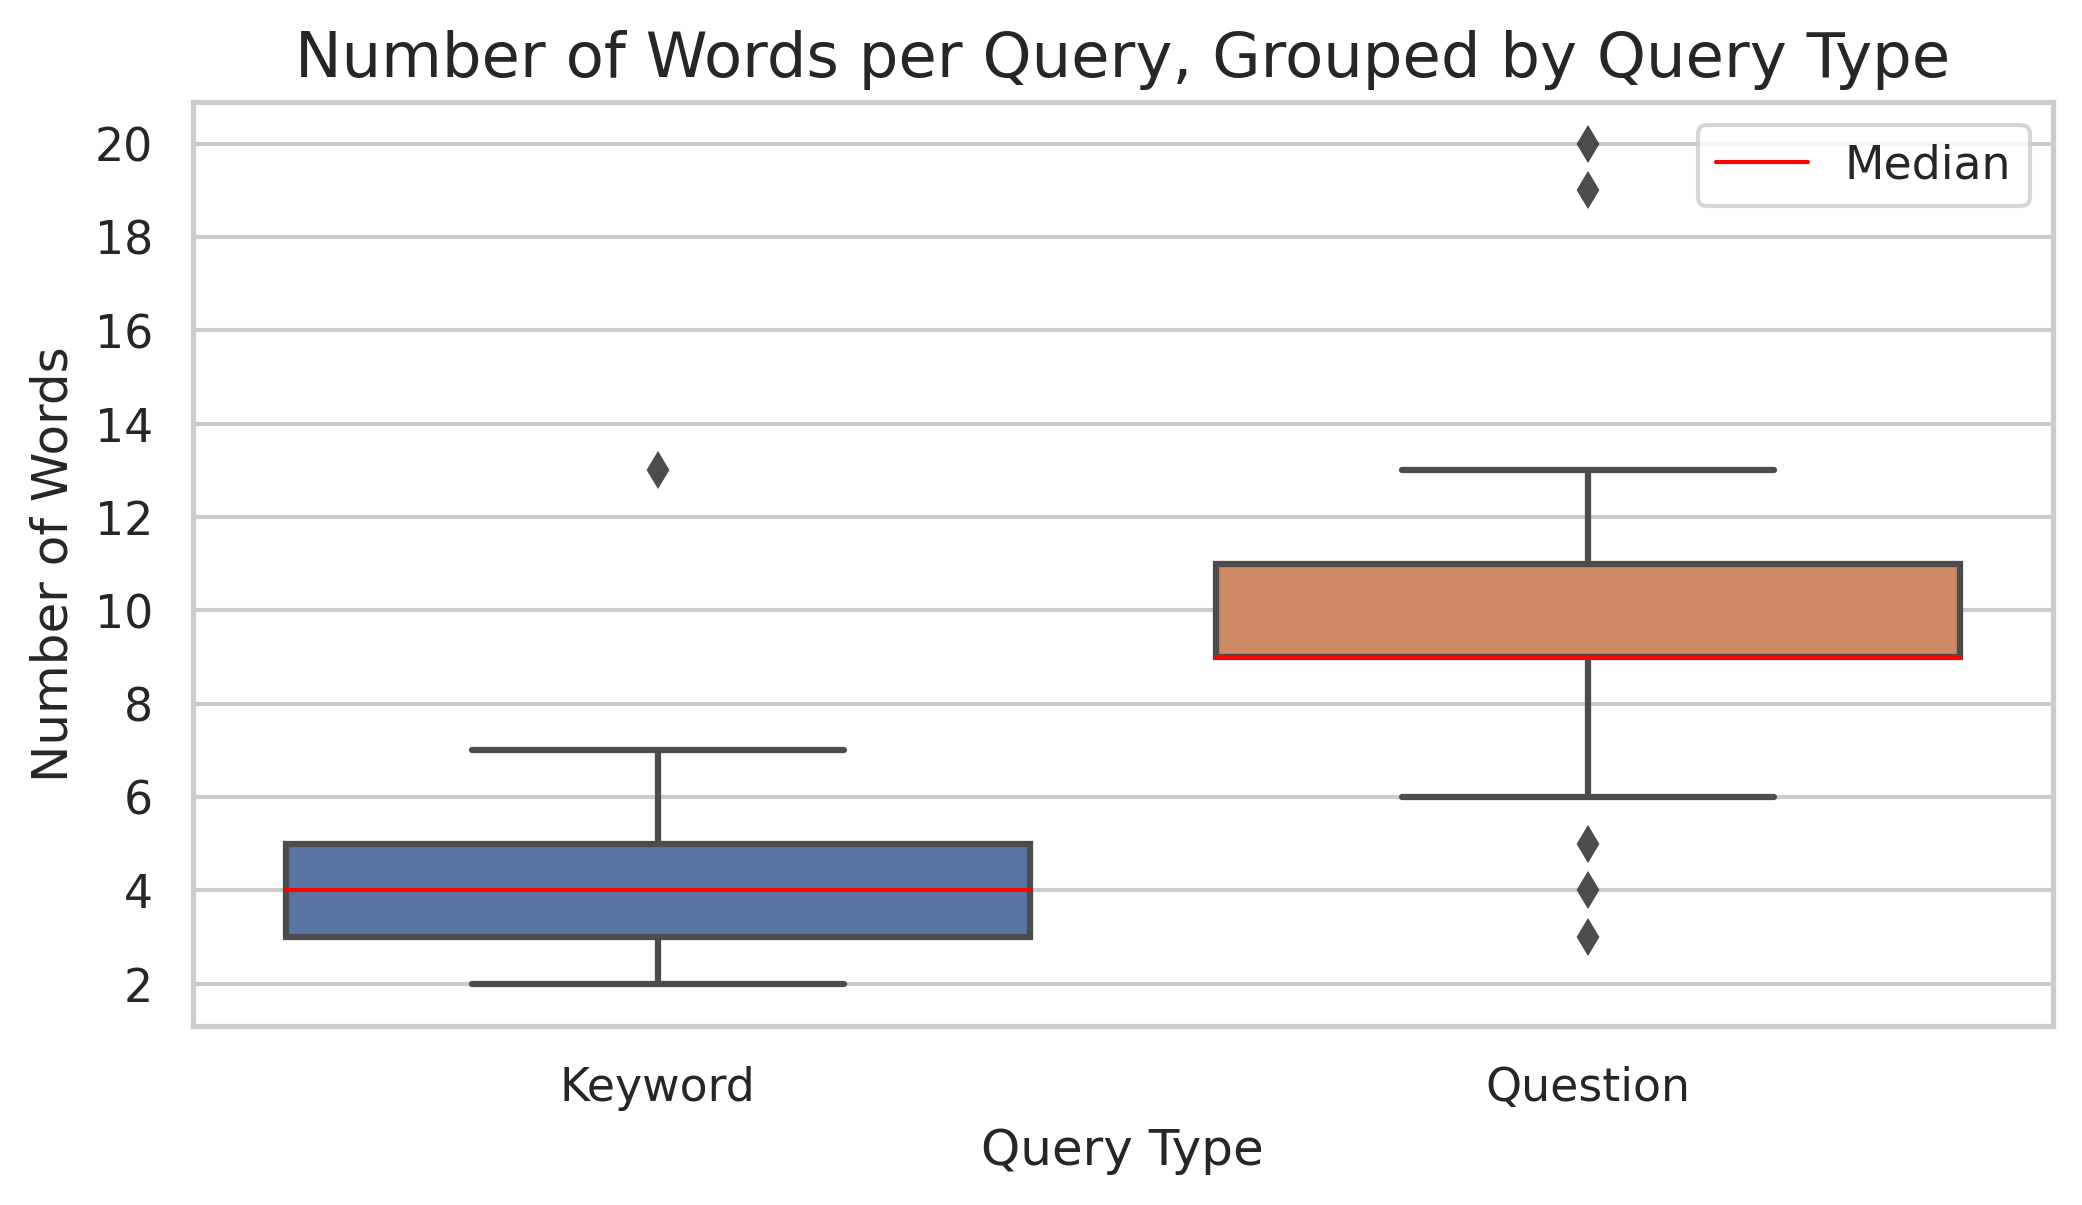
\includegraphics[width=\textwidth]{images/num_words_per_query.png}
\caption{Boxplot of the number of words per query, split by query type. Keyword queries are shorter than question queries with a median of 4 words compared to 7 words for the question queries.}
\label{fig:num_words_per_query}
\end{figure}
In total, we identify 17 question-style queries and 33 keyword-style queries.
Figure \ref{fig:num_words_per_query} shows the number of words per query for both query types.
As expected, the keyword queries are shorter than the question queries, with a median of 4 words compared to 7 words for the question queries.
The shortest query is only two words long, while the longest query is 20 words long.
\subsection{Documents}
\begin{table}[tb]
\centering
\begin{tabular}{ll}
\hline
\textbf{Domain} & \textbf{Occurrences} \\
\hline
www.healthline.com & 603 \\
www.nationalmssociety.org & 419 \\
www.ms.org.au & 198 \\
jhu.pure.elsevier.com & 191 \\
www.msif.org & 183 \\
www.psychologytoday.com & 161 \\
www.urotoday.com & 155 \\
www.news-medical.net & 150 \\
www.sleepfoundation.org & 141 \\
www.aafp.org & 139 \\
\hline
\end{tabular}
\caption{Top 10 Most Frequently Occurring Domains}
\label{tab:top_domains}
\end{table}
The documents in the dataset are scraped from a total of 234 different domains.
Table \ref{tab:top_domains} shows the top 10 most frequently occurring domains in the dataset.
Most domains are health related, belonging to either health organizations, medical journals or health news websites.
Some domains are more general, e.g. there are also wikipedia.org pages in the dataset, as well as some domains from essay writing or homework help websites.
A total of 133 domains show up less than 10 times in the dataset, while 44 domains show up only once.
\\\\
\begin{figure}[tb]
\centering
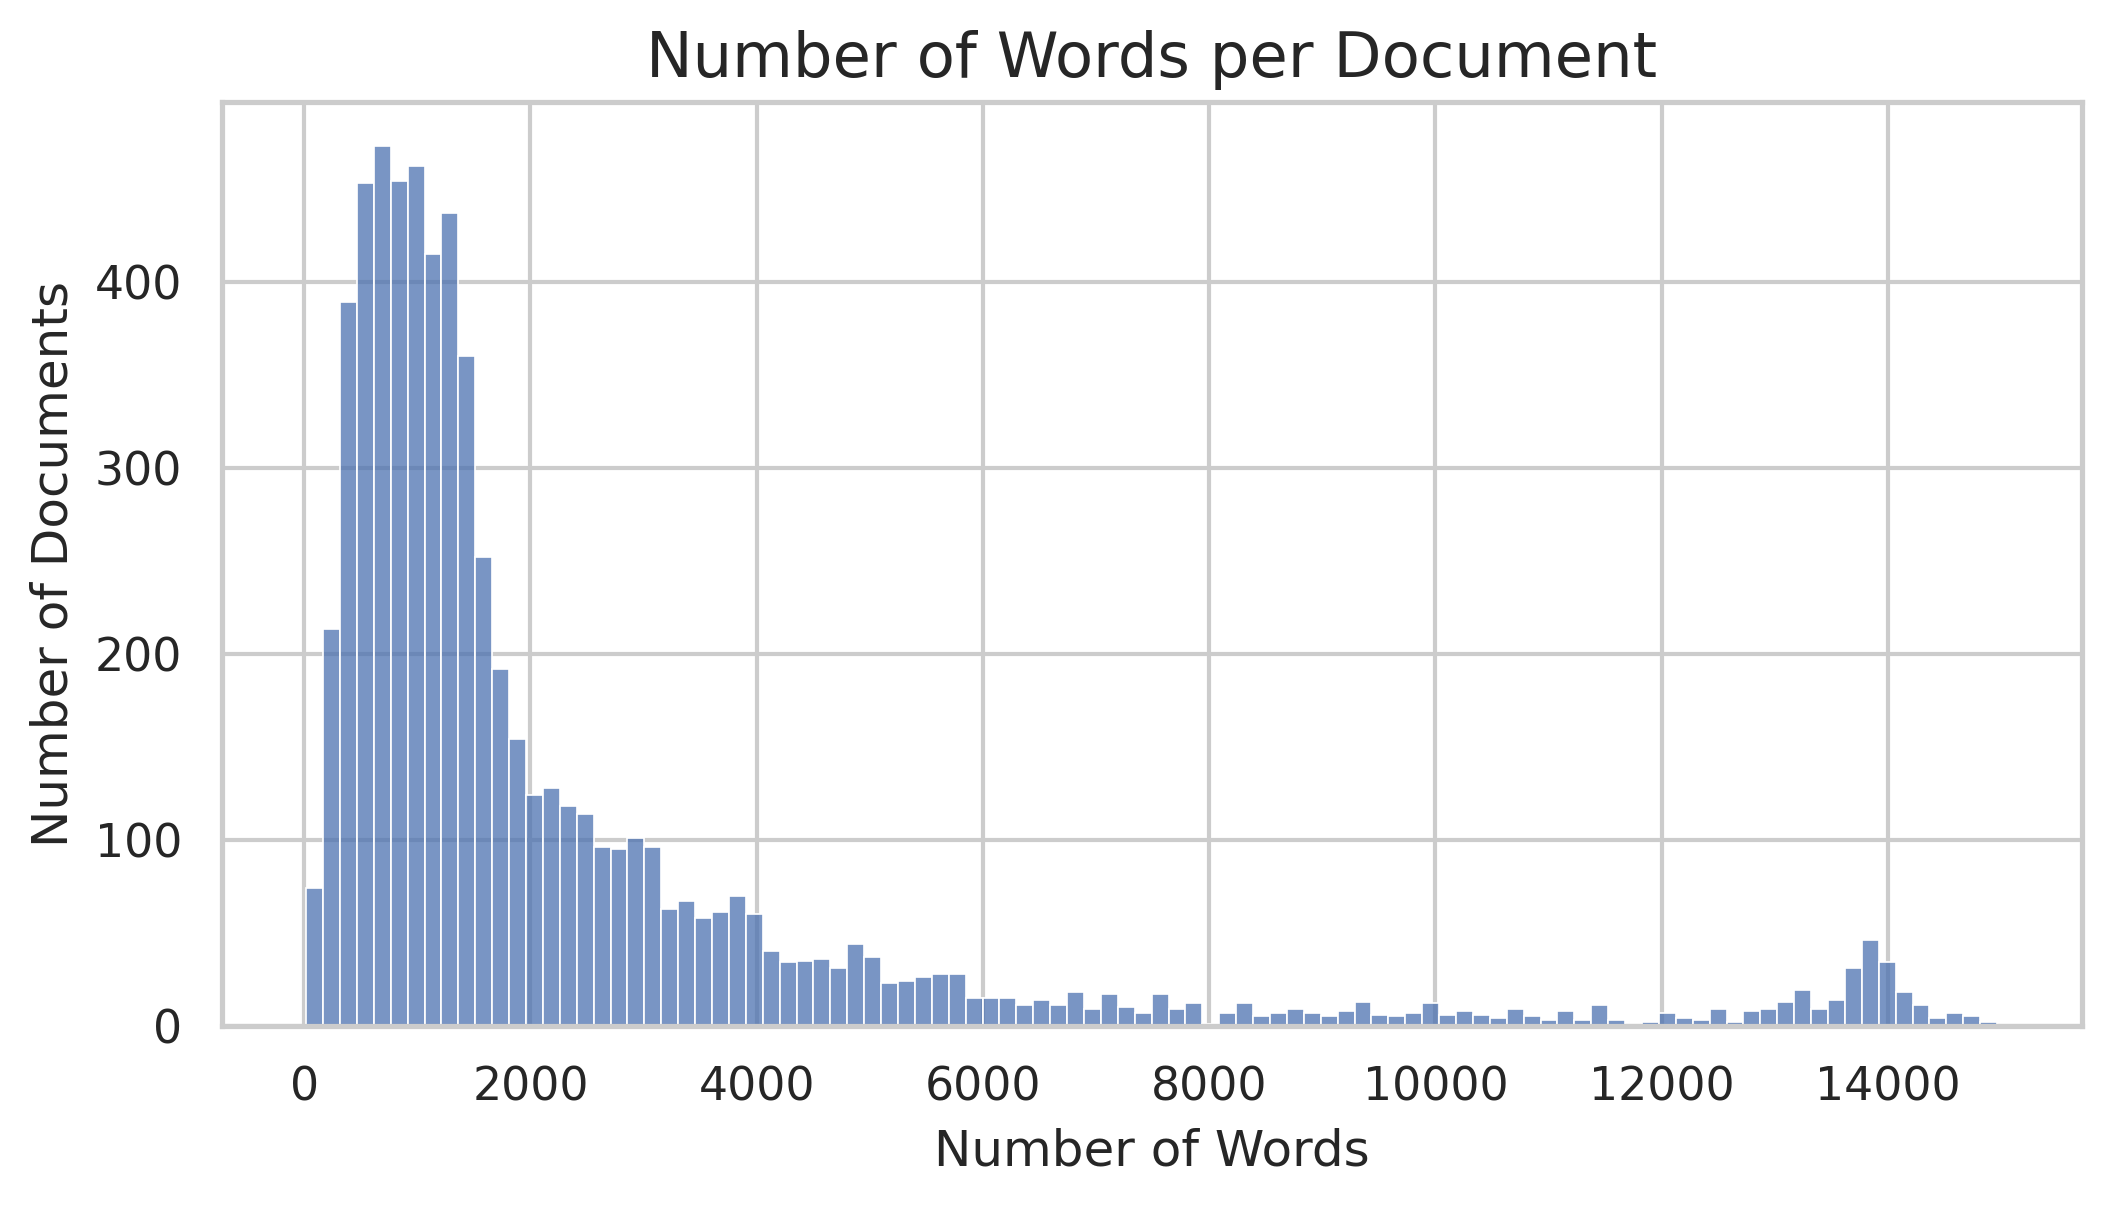
\includegraphics[width=\textwidth]{images/num_words_per_passage.png}
\caption{Histogram of the number of words per document. The plot is cut at 15 000 words, which excludes 120 or 2\% of the documents. The median number of words per document is 1354, while the mean is 2901.}
\label{fig:num_words_per_document}
\end{figure}
After preprocessing, the documents are cleaned of all HTML tags and of HTML elements containing fewer than 50 characters.
Figure \ref{fig:num_words_per_document} shows that the number of words per document is very high, with a median of 1354 words and a mean of 2901 words.
This is natural for documents scraped from the web, which do not only contain the main text, but also navigation bars, footers, sidebars and other elements.
Those can not be fully removed with our trivial preprocessing methods.
\subsection{Document Metrics}
The document metrics in the dimensions of readability, credibility and relevance are based on the human annotations from \cite{goeuriot:2021}.
In general, a surprisingly high number of documents are rated as not relevant to the given query.


\section{Retrieval Pipelines}

\section{Ranking of Generated Answers}
% 
\chapter{Discussion}\label{discussion}

In this chapter, we discuss the results of our experiments and their implications for the research questions. 

\section{RQ1: Factors Influencing LLM Effectiveness}

The effectiveness of LLMs in providing health-related answers varies significantly depending on several factors, as shown by our experimental results.

\subsection{Model Size}
Our results show a strong connection between model size and ranking results in our retrieval-based implicit evaluation as evident in Figure \ref{fig:weighted_position_vs_model_size}. 
Especially the differences between the GPT-2 based models are insightful, as they share the same architecture and dataset, only differing in the number of parameters.
The larger the model size, the better the ranking results, which aligns with the findings of \cite{radford:2019:language} who showed that the increased model sizes leads to better performance on various NLP tasks.

With 185 billion parameters, ChatGPT is the largest model in our evaluation, and it ranks best on nearly every query.
For the small to medium-sized fine-tuned models, specifically the 7B variant of Falcon and the 7B and 13B variants of Llama-2, the trend is less clear.
Llama-2 7B performs better than the 7B variant of Falcon, scoring a mean normalized rank of 0.079 compared to 0.146 by Falcon 7B.
Even though they have the same number of parameters, the differences could be explained by the different training data used for the models and the more sophisticated fine-tuning strategy of Llama-2.

More surprisingly, Llama-2 7B on average ranks about as well as its larger variant, which has nearly twice as many parameters.
This indicates either a saturation of the model's effectiveness or that the ranking result is not accurate enough to distinguish between the two models.
Since according to the original paper \cite{touvron:2023:Llama} the model exhibits the usual trend of increasing performance with model size, we assume that the latter is the case.

So, while the model size is a strong indicator of the model's effectiveness in our evaluation, the results do not fully align with the expected trend.

\subsection{Prompting Strategy}
Prompting strategies have a significant impact on the effectiveness of LLMs, shown in Table \ref{tab:prompting_strategy}.
There is a general tendency that the more sophisticated the prompting strategy, the better the ranking results.
While there are two outliers (GPT-2 Medium and GPT-2 Large), which rank better with one of the simpler prompting strategies, the overall trend is clear, with the MultiMedQA prompt leading to the best results.
This aligns with the findings of \cite{reynolds:2021:Prompt} who showed this pattern for the task of text translation using GPT-3.

Even for ChatGPT, which already ranks best on nearly every query without any additional prompting, the ranking results are best when using the complex MultiMedQA prompt.
We assume the small differences between the prompting strategies are due to the fact that the models are already very effective in answering the queries, so the additional prompting does not have a large impact.

Except for ChatGPT, all models perform worse than the next smaller model, if the smaller models uses the MultiMedQA prompt and the larger model uses no additional prompting.
This emphasizes the importance of a good prompting strategy, even for models that are already fine-tuned for a conversational experience like Falcon and Llama-2.

\subsection{Query Type}
Similar to the influence of prompting strategies, our results show that phrasing the query as a proper question leads to better ranking results than using a keyword-based query.
The improvements are consistent across all models, but the difference seems to be less pronounced the larger the model is, as shown in Figure \ref{fig:weighted_position_boxplot_by_model_and_question}.


\subsection{Lower ranked Answers Properties}
When investigating why certain answers by ChatGPT are ranked especially low, we found that the lower ranked answers follow two patterns.
They either contain the phrase ``As an AI..'' or they contain a formatted list.
For both patterns, we investigated if they are also present in other LLMs and how they are ranked.

The substring ``As an AI..'' is present in answers generated by ChatGPT and by Falcon 7B, but not in any of the other models.
The phrase is commonly used by ChatGPT and seems to be a part of OpenAI's training data, leading the model to not answer controversial questions or telling the user that it does not have enough information to provide an answer.
As Falcon 7B's training data is in part based on self-chats of ChatGPT(see Section \ref{sec:dialog-models}), it is not surprising that it also uses this phrase.
Answers containing this substring are ranked lower than other answers, which indicates that the ranking pipeline works as expected in this case, as the answers most likely are not useful for the user.
On the other hand, telling the user that the model is unable to answer the question should be considered a desirable behavior, as the alternative would be to provide a misleading answer.
Future research in retrieval-based implicit evaluation should investigate how this behavior could be evaluated

Answers exhibiting the list pattern are generated by all models, except for GPT-2 and GPT-2 Medium.
There seems to be a connection between the model size and the frequency of this pattern, as the larger models generate more answers containing lists.
The effect of achieving a worse ranking by using this pattern is not consistent over all models, as the Llama-2 models answers perform better when using this pattern.
Additionally, many highly ranked answers by ChatGPT also contain lists, so the pattern is not a clear indicator of a bad answer.
We assume that observing this pattern in many of the lower ranked answers is dependent on the queries that prompted the answers, which are all keyword-based queries.
This is consistent with the previous finding that keyword-based queries lead to worse ranking results than question-type queries.

\subsection{Answer Length}
FIgure \ref{fig:weighted_position_vs_answer_length} shows that there is a connection between the length of the generated answer and the ranking result.
Very short and very long answers are ranked worse than answers of medium length containing between 200 and 300 words.
Short answers being ranked worse is consistent with expectations, as the often complex questions require longer answers to be answered sufficiently.
Longer answers being ranked worse is more surprising, but closer inspection revealed that most of the overly long answers are generated by GPT-2 variants, explaining the worse ranking results.
This could potentially be avoided with other parameters used for the generation, but we did not investigate this further.

\section{RQ2: Comparison with Other Benchmarks}
Comparing the results of our retrieval-based implicit evaluation with other benchmarks, proved to be challenging, as there are no other benchmarks for evaluating LLMs in the context of LFQA.



\section{Is the Proposed Retrieval-Based Evaluation Effective?}


% \chapter{Future Work and Conclusion}\label{conclusion}

\section{Future Work}
In this thesis, we present a first approach to using IR methods for evaluating LLMs in LFQA, specifically in the medical domain.
However, there is substantial room for further research and development.
Some areas on which future work could focus are:

\begin{enumerate}
    \item \textbf{Dataset Quality:} The currently used dataset is not originally designed for LFQA and has some limitations, as discussed in Chapter \ref{sec:scope-and-limitations}. Those limitations include the generally lower quality of web content as well as the problems in the annotation process. Future work could focus on designing a more comprehensive dataset that addresses these limitations and provides a more challenging benchmark for LLMs. An intermediate step could be to use the existing dataset and incorporate more sophisticated preprocessing steps to improve the quality of the data. Redoing the current annotations using a more consistent methodology could also improve the dataset quality.
    \item \textbf{Retrieval Pipeline Improvements:} The retrieval pipeline used in this thesis is a first attempt at using IR methods for evaluating LLMs in LFQA. Future work could focus on improving the pipeline's performance and investigate closely in which cases the retrieval pipeline does not align with human annotator preferences. 
    \item \textbf{Multidimensional Evaluation:} The currently used retrieval pipeline is only trained to rank documents based on their relevance, which is only one of the dimensions of answer quality. Future work could focus on extending the pipeline to rank documents based on their readability and credibility.
    \item \textbf{Human Evaluation:} The chosen retrieval pipeline is evaluated on the human-ranked documents from the dataset, but after including the LLM-generated answers the produced ranking is not reevaluated by medical experts. Future work could evaluate if human experts prefer the highest-ranked LLM-generated answers over the highly ranked web answers.
    \item \textbf{Conversational LLMs:} As the current application of LLMs in chatbots is focusing on conversational experiences, it is important to consider the evaluation of these systems, which is more complex than the evaluation of single answers. A first step could be to concatenate the generated answers over multiple conversation turns and rank this against the web document, essentially evaluating the generated text as a whole.
\end{enumerate}

\section{Conclusion}
In this thesis, we present a first approach of using human-written web content as a proxy for evaluating LLMs in LFQA, specifically in the health domain.
We propose a rank-based implicit evaluation method that uses IR methods to rank documents based on their relevance to the question.
Our contributions are:
\begin{enumerate}
    \item Adapting the existing dataset by \cite{goeuriot:2021:Consumer} to the LFQA task.
    \item Implementing and evaluating different retrieval pipelines for the new dataset.
    \item Producing a supplementary dataset of 16,000 answers for the queries in the dataset, using multiple LLMs and prompting strategies.
    \item Evaluating the LFQA performance of the LLMs using the most effective retrieval pipeline.
    \item Investigating which factors influence the ranking of the LLM-generated answers.
    \item Comparing the effectiveness of LLMs on our benchmark to the effectiveness on other benchmarks.
\end{enumerate}

Although the dataset we adapted for this task has several limitations preventing it from being a challenging benchmark that allows for fine-grained evaluation of LLMs, this thesis lays the groundwork for a scalable evaluation method for LFQA.
The proposed rank-based implicit evaluation method is a solid foundation for future work, which could focus on improving the retrieval pipeline, extending the evaluation to other dimensions of answer quality, and creating a more challenging dataset.

% Bibliography
\bibliographystyle{apalike} % requires package natbib. An alternative is apalike
\bibliography{literature}    % load file literature.bib

% \appendix
\chapter{My First Appendix}
This was just missing.


\end{document}

